\documentclass[12pt,a4paper]{article}

% "Vorgegebene packages"
\usepackage{a4wide}
%\usepackage{fancyhdr} % delete this, I prefer "scrlayer-scrpage"
\usepackage{tikz} % other cool packages?
\usepackage{graphicx}
\usepackage{floatflt, epsfig}
\usepackage{float} % allows for the usage of \begin{figure}[H] to specify "in-text-floating"
\usepackage{subcaption} % use subcaptions in subfigures
\usepackage{parskip}
\usepackage[utf8]{inputenc}
\usepackage{amsmath}
\usepackage{amssymb}
\usepackage{mathtools} % better text over arrow
\usepackage{bm}
\usepackage{subcaption}
\usepackage[free-standing-units=true]{siunitx} % for consistent handling of SI units
\usepackage[colorlinks=true, pdfstartview=FitV, linkcolor=blue, citecolor=blue, urlcolor=blue]{hyperref} % enable links

% My own additions
\usepackage{enumerate} % to enable i, ii, iii enumeration
\usepackage{hyperref} % to be able to click on links in PDF (nice to have)
\usepackage[style=numeric, backend=biber]{biblatex} % better source handling % alphabetic
\bibliography{literature.bib} % Enables an external sources document to be read in
\usepackage[format=hang,
            font=footnotesize,
            labelfont={bf,it},
            textfont=it,
            justification=RaggedRight,
            singlelinecheck=false]{caption} % better label-formatting
%\setcounter{biburlnumpenalty}{7000} % To enable linebreaks in long urls for numbers

\nocite{*} % Displays all sources at once without having to “quote” first
\usepackage{pdfpages} % Simple attachment of pdf files (such as measurement report)
\usepackage{makecell} % Line breaks within tables

% The following paragraph contains stuff to display code nicely
\usepackage{listings}
\definecolor{codegreen}{rgb}{0,0.6,0}
\definecolor{codegray}{rgb}{0.5,0.5,0.5}
\definecolor{codepurple}{rgb}{0.58,0,0.82}
\definecolor{backcolour}{rgb}{0.95,0.95,0.92}
\lstdefinestyle{mystyle}{
    backgroundcolor=\color{backcolour},   
    commentstyle=\color{codegreen},
    keywordstyle=\color{magenta},
    numberstyle=\tiny\color{codegray},
    stringstyle=\color{codepurple},
    breakatwhitespace=false,     
    basicstyle=\ttfamily\scriptsize,
    breaklines=true,                 
    captionpos=b,                    
    keepspaces=true,                 
    numbers=left,                    
    numbersep=5pt,                  
    showspaces=false,                
    showstringspaces=false,
    showtabs=false,                  
    tabsize=2
}
\lstset{style=mystyle}


%Kopfzeile (design-Vorschlag)
\usepackage[headsepline]{scrlayer-scrpage}
\newpairofpagestyles{trueempty}{
    \ihead{\section*{Appendix}}
    \KOMAoption{headsepline}{false} % Deactivates the header line for appendix
}% define a new but empty pair of page styles headings and plain
\pagestyle{scrheadings}
\clearscrheadfoot
\automark[section]{section}
\cfoot{\pagemark}
\ohead{} % 
\ihead{DSMC for Coulomb Collisions\\\leftmark} % statt \ohead{Physics Lab I\\Experiment October 15, 2021} 


% Other mathematical additions
\usepackage{physics} % Other mathematical additionsThe most important package for writing fractions/matrices/derivations/... to write. Instructions: http://mirrors.ibiblio.org/CTAN/macros/latex/contrib/physics/physics.pdf
%\usepackage{comment} % allow comment environment
\usepackage{algorithm,algorithmic} % for nice box around algorithm

\setlength{\parindent}{0pt} % Sets the indentation after a “real paragraph” to 0

\newcommand{\m}[1]{\mathrm{#1}} % Shortcut for bold formulas (such as $\m{F}$, which makes “F” bold)

%\author{Alexander Liemen}
\date{\today}

\begin{document}

\begin{titlepage}
\title{
    \vspace*{-3cm}  
    \begin{figure}[H]
        
\includegraphics[scale=0.65]{ressources/logos/ethlogo_full.pdf}
        \hfill
        
\includegraphics[scale=0.4]{ressources/logos/psi_logo_blue.pdf}
    \end{figure}
    \begin{tikzpicture}
        \draw[very thick] (0,0) -- (\textwidth,0);
    \end{tikzpicture}
    \bfseries {\\\huge \sc{Direct Simulation Monte Carlo Methods Adapted for Coulomb Collisions}}
    \begin{tikzpicture}
        \draw[very thick] (0,0) -- (\textwidth,0);
    \end{tikzpicture}
}
\author{
        \textsc{{{Semester Project}}} \\[5pt] 
        \small ETH Zurich \vspace{0.4cm} \\[0.2in]
        \\ \small written by \\[5pt]
        %\small \sc{BSc ETH xxx} \\
        \begin{minipage}[h]{\linewidth}
            \centering
            \begin{tabular}{r|l}
                \sc{Alexander Liemen} & \href{mailto:alexander.liemen@inf.ethz.ch}{alexander.liemen@inf.ethz.ch} 
            \end{tabular}
        \end{minipage} 
        \vspace{1cm} \\
        \small supervised by \\[5pt]
        Dr.\ Andreas\ Adelmann \\
		\vspace{0.5cm} \\
        \small scientific adviser \\[5pt]
        Dr.\ Sadr\ Mohsen \\
        \vspace{1.5cm} \\
        \today
}
\date{}
% \clearpage
%\maketitle
\thispagestyle{empty}
\end{titlepage}

\maketitle


\newpage
\thispagestyle{empty}
\begin{abstract}\label{abstract}
    This project focuses on simulating the relaxation behavior of a charged plasma, typically composed of electrons, using a particle-based approach. 
    %Plasma simulations have wide ranging applications, including advancements in particle accelerator technology, plasma-light interactions, and space propulsion systems. Among the various simulation methods, 
    This study employs the Direct Simulation Monte Carlo (DSMC) approach to address the computational challenges inherent in solving kinetic equations for plasmas. The implementation leverages the IPPL (Independent Parallel Particle Layer) framework and evaluates two collision algorithms, proposed by \textsc{Takizuka} and \textsc{Abe} (TA), and \textsc{Nanbu}. \\
    IPPL allows the algorithm to be fast and scalable. Both algorithms are benchmarked using three tests: the \textsc{Trubnikov} test to evaluate the collisions, the relaxation of a delta-like initial distribution and the induced heating of a cold sphere. \\
    Overall, the project concludes that \textsc{Nanbu}'s algorithm (1997) does not provide a significant advantage over TA (1977) in its proposed implementation due to its increased computation time caused by the need to solve an additional equation. However, further improvements are addressed at the end.
\end{abstract}

\newpage
\tableofcontents

\newpage
\section{Introduction}

% We consider systems of charged particles that interact through Coulomb force. This types of systems can be, for instance, encountered in plasmas. The goal of this project is to investigate such systems out of their equilibrium and simulate their evolution. 

% In order to do that, short-range and long-range interactions have to be considered separately. Short-range interaction are represented as Coulomb collision. They can be  simulated through a modified direct simulation Monte Carlo method. In this project, we consider the Nanbu-Bobylev \cite{bobylev_nanbu}, Nanbu-Babovski and Bird algorithm \cite{dimarco2010direct}.
% And we use a particle-mesh solver with an electric field to compute long range interactions.
% Then, we consider different test cases to determined the efficiency and accuracy of the models.
% test \cite{medaglia2024particle}

% - This project aims to simulate the relaxating behaviour of a charged plasma (usually electrons, but it is applicable for every charged particle cloud).
% - Modern Physics has many applications for accurate simulations of a plasma (advancing particle accelerator technology, plasma-light interactions or even space propulsion \cite{wikipedia_plasma_propulsion}).
% - Many possibilities to do such a simulations: solving kinetic equations by discretizing on a grid (Eulerian approach), treating the plasma as a fluid (magnetohydrodynamics) or some combinations. 
% - This project uses a particle based approach. Solving equations is computationally intense: use a Monte-Carlo approach. Use an electric field solver for kinetic advancement and use a statistical approach to the collisions to significantly reduce computation.
% - All this is done using the IPPL framework \cite{muralikrishnan2024scaling}.
% - Important for this project: the Monte-Carlo part for the collisions. Compare two different algorithms from Takizuka \& Abe \cite{TakizukaAbe1977} and Nanbu \cite{Nanbu1997} in terms of accuracy, efficiency and scalability.

This project aims to simulate the relaxing behavior of a charged plasma, typically consisting of electrons, although the methods are applicable to any charged particle cloud. Accurate plasma simulations have numerous applications in modern physics, ranging from advancing particle accelerator technology and understanding plasma-light interactions to even enhancing space propulsion systems \cite{wikipedia_plasma_propulsion}.

There are several approaches to simulating a plasma. One method involves solving kinetic equations by discretizing them on a grid, known as the \textsc{Eulerian} approach. Another treats the plasma as a fluid, which falls under magnetohydrodynamics. Additionally, various combinations of these methods exist. This project, however, employs a particle-based approach. Given the computational intensity of solving equations in this context, we utilize a \textsc{Monte-Carlo} method. This involves an electric field solver for kinetic advancement and a statistical approach to handling collisions, which aims to significantly reduce computational demands.

The implementation of these methods is carried out using the IPPL framework \cite{muralikrishnan2024scaling}. A crucial aspect of this project is the \textsc{Monte-Carlo} component for simulating collisions. Specifically, we compare two different algorithms -- those proposed by \textsc{Takizuka} and \textsc{Abe} \cite{TakizukaAbe1977}, and \textsc{Nanbu} \cite{Nanbu1997} -- in terms of their accuracy, efficiency, and scalability.

By evaluating these algorithms, this project aims to identify an effective method for scalable plasma simulations, contributing to the broader field of plasma physics and its many applications. All code referenced in the following can befound in \cite{aliemen2024}.


\section{Theory Background and Algorithms}

% This part described the theoretical background of the different used methods. 
% As the Coulomb force is an long range interaction, we split the schemes in one part focusing on short-range interactions, and one on long-range interactions. Long-range interactions can be solve using the Poisson equation, by considering the electric field resulting from the distribution of the particles.

% The following part of this section focuses on the short-range interaction. More precises construction can be find in \cite{rosenbluth}, \cite{bobylev_nanbu} and \cite{dimarco2010direct}.

% Both methods mentioned in the introduction are based on the 
%- As mentioned, the final simulation for non-equilibrium states consists of a field solution as well as the collisions. However, solving the field is part of the investigation, since it is already implemented by IPPL and the same for both models.
%- The field solver and how it it implemented will be explained briefly at the end of this section. 
%- In the following, a rough outline of the most important equations and approximations used by the two collision algorithms mentioned is given. 

As mentioned, the final simulation for non-equilibrium states consists of both a field solution and the statistical modeling of collisions. The field solution, which is already implemented by the IPPL (Integrated Plasma Physics Library), is a crucial part of the later investigation, but remains the same across both models. Therefore, the core of this discussion will be dedicated to outlining the most important equations and approximations used by the two collision algorithms. \\
The field solver and its implementation will be briefly explained in \ref{sec:FieldSolverImplementation} to provide context. 


\subsection{\textsc{Boltzmann} and \textsc{Fokker-Planck} Equation}

To derive the Direct Simulation \textsc{Monte-Carlo} methods (in the following refered to as DSMC), the plasma is conveniently described as a particle distribution function $f_a(x^\mu, v^\mu)$, which described the number of particles of species\footnote{The test cases only deal with one species. Since everything also works with multiple species, the index $a$ is used in the theory explanation.} $a$ per volume in phase space. $x$ denotes position, $v$ velocity.

The underlying equation to describe the behaviour of a distribution function $f$ is the \textsc{Boltzmann} equation \cite[1]{Rosenbluth1957}:
\begin{equation*}
    \pdv{f_a}{t} + v^\mu \pdv{f_a}{x^\mu} + \frac{F^\mu}{m} \pdv{f_a}{v^\mu} = \qty(\fdv{f_a}{t})_\mathrm{c}
\end{equation*}
with particle mass $m$ and external force field $F$. Since we consider the electromagnetic field, we can insert the Lorentz force and rewrite it in terms of vectors:
\begin{equation*}
    \pdv{f_a}{t} + \mathbf{v} \cdot \nabla_x f_a + \frac{e_a}{m_a} \qty(\mathbf{E} + \mathbf{v} \times \mathbf{B}) \cdot \nabla_v f_a = \qty(\fdv{f_a}{t})_\mathrm{c} .
\end{equation*}

$\qty(\fdv{f_a}{t})_\mathrm{c}$ describes the change of the distribution due to collisions, which can be calculated. Since inverse square laws have significant long-range interaction, we can assume that small angle collisions are the most probable, which leads to the following term in second order (component-wise notation) \cite[2]{Rosenbluth1957}:
\begin{equation}
    \qty(\fdv{f_a}{t})_\mathrm{c} = - \pdv{v^\mu} \qty(f_a \expval{\Delta v^\mu}_a) + \frac{1}{2} \pdv{}{v^\mu}{v^\nu} \qty(f_a \expval{\Delta v^\mu \, \Delta v^\nu}_a) , \label{eq:2.1:fokkerplanck_base}
\end{equation}
where $\expval{\Delta v}$ stands for the mean velocity increment per time.

Assuming that changes in velocity happen due to binary particle interactions, the expectation values can be calculated according to \cite[2]{Rosenbluth1957} using the following differential cross section:
\begin{equation*}
    \sigma\qty(\Omega) = \frac{e_a^2 e_b^2}{4 m_{ab}^2 u^4} \sin^{-4} \qty(\frac{\Theta}{2}) ,
\end{equation*}
where $a$, $b$ denote the different species included in the collision, $e$ stands for the charge, $m_{ab} = \frac{m_a m_b}{m_a+m_b}$ is the reduced mass, $\Theta$ the scattering angle and $u$ the absolute relative velocity between both particles. This gives the following collision operator and defines the \textsc{Fokker-Planck} equation together with \eqref{eq:2.1:fokkerplanck_base} according to \cite{Wang2008} in the \textsc{Landau} form:
\begin{equation}
    \qty(\fdv{f_a}{t})_\mathrm{c} = - \sum_b \pdv{v_j} \frac{e_a^2 e_b^2 \,\ln\Lambda}{8 \pi \epsilon_0^2 m_a} \, \int \, \dd v^\prime \qty[\frac{\delta_{jk}}{u} - \frac{u_j u_k}{u^3}] \qty[\frac{f_a}{m_b} \pdv{f_b\qty(v^\prime)}{v_k^\prime} - \frac{f_b}{m_a} \pdv{f_a\qty(v^\prime)}{v_k}] , \label{eq:2.1:LandauFokkerPlanckOperator}
\end{equation}
where $\ln\Lambda$ is the \textsc{Coulomb} logarithm\footnote{This parameter is calculated from the \textsc{Debye} length $\lambda_\mathrm{D}$, which intuitively describes the cutoff around the electron until which collisions are significant. There is a formula that can be used to calculate the \textsc{Coulomb} logarithm. However, since this contains the temperature, the calculation might get computationally intense for very small gain. So, it is better to simply use $\ln\Lambda = 10$ from now on according to \cite{fitzpatrick_coulomb_logarithm}.}.

Treating the distribution $f$ as a sum of discrete particles, the integral in \ref{eq:2.1:LandauFokkerPlanckOperator} can be solved. Then, after discretizing $\qty(\fdv{f_a}{t})_\mathrm{c}$ and equation \eqref{eq:2.1:fokkerplanck_base} in time, we can solve for $f^{t + \Delta t}$ and get the update equations outlined in \ref{sec:TA_updateEQ} and \ref{sec:Nanbu_updateEQ}.


\subsection{Algorithm Outline}

The general method is the same for both algorithms: First, the field solver is executed to determine the self consistent electric fields. Then, collision pairs are selected based on the specific algorithm being employed. Following this, binary collision updates are calculated for the selected pairs. Finally, a leap-frog integration step is utilized to advance the particles' positions and velocities, taking into account both the calculated electromagnetic fields and the newly computed velocities from the collision updates. This basic outline of the simulation process is illustrated in algorithm \ref{algo:2.2:GeneralPlasmaSimulation}. \\
\begin{algorithm}[H]
\caption{General Simulation Step}\label{algo:2.2:GeneralPlasmaSimulation}
\begin{algorithmic}[1]
    %\scriptsize
    \STATE Select $\Delta t$
    
    \texttt{\\/* First, the electric field is calculated on a grid. Then the grid can be used to interpolate the field values onto the particle positions. */}
    \STATE $E \leftarrow$ runFieldSolver($f$)
    \STATE pairs $\leftarrow$ selectCollisionPairs($f$)
    \FOR{Every Particle Pair $(i, j)$}
        \STATE $\Delta v \leftarrow$ getCollisionUpdate($i$, $j$) 
        
        \texttt{\\/* Advance every particle by $\Delta t$, assume $m_a=m_b$. */}
        \STATE $v_{i, j} \leftarrow v_{i, j} \pm \frac{\Delta v}{2}$ 
    \ENDFOR

    \texttt{\\/* Do a leap-frog step (every operation performed particle-wise). */}
    \STATE $v \leftarrow v + \frac{\Delta t}{2} \cdot \frac{e}{m} \cdot \frac{E}{\epsilon_0}$ \texttt{// Kick 1}
    \STATE $x \leftarrow x + v \cdot \Delta t$ \texttt{// Drift}
    \STATE $v \leftarrow v + \frac{\Delta t}{2} \cdot \frac{e}{m} \cdot \frac{E}{\epsilon_0}$ \texttt{// Kick 2}

    \texttt{\\/* Update how particles are distributed onto the computational grid in IPPL. */}
    \STATE particleNodeDistributionUpdate()
\end{algorithmic}
\end{algorithm}
This demonstrates that the primary distinction between the algorithms lies in the selection of particle pairs for the collision step and the method used to calculate the velocity updates for each pair. These specifics are explained in the following two sections.


\subsection{Takizuka and Abe's (1977) Collision Model}\label{sec:TA_updateEQ}

\textbf{Selecting the particle pairs.} This algorithm uses all available particle pairs. From the $N$ particles, $\frac{N}{2}$ pairs are selected (assuming an even number of particles), where every particles collides exactly once. 

\textbf{Calculating the velocity update.} Next, $\Delta v$ mentioned in the algorithm \ref{algo:2.2:GeneralPlasmaSimulation} is calculated according to \cite[4310]{Wang2008}:
\begin{itemize}
    \item Assume two particles $i$ and $j$ with their respective masses, charges, number density $n$ (the same for both particles) and relative velocity $\mathbf{u} = \mathbf{v}_i - \mathbf{v}_j$ and reduced mass $m_{ij}$. Also:
    $$
    \mathbf{u} = \mqty(u_x\\u_y\\u_z) ,
    \qquad u_\perp = \sqrt{u_x^2 + u_y^2}
    $$
    \item Calculate the variance
    $$
    \expval{\delta^2} = \frac{e_i^2e_j^2n \,\ln\Lambda}{8\pi\epsilon_0^2m_{ij}^2u^3} \cdot \Delta t
    $$
    and sample the variable $\Phi$ normally distributed around mean 0 and with variance $\expval{\delta^2}$. 
    \item Sample the angle $\Theta$ uniformly distributed between $0$ and $2\pi$.
    \item Use the angles to calculate the $\cos$ and $\sin$:
    $$
    \sin\Theta = \frac{2 \delta}{1 + \delta^2}, \qquad \cos\Theta = 1 - \frac{2 \delta^2}{1 + \delta^2}. 
    $$
    \item Finally use everything to calculate the velocity update:
    $$
    \Delta \mathbf{v} = \mqty(\frac{u_xu_z}{u_\perp}\sin\Theta\cos\Phi - \frac{u_yu}{u_\perp} \sin\Theta\sin\Phi \\
                              \frac{u_yu_z}{u_\perp}\sin\Theta\cos\Phi - \frac{u_xu}{u_\perp} \sin\Theta\sin\Phi \\
                              -u_\perp\sin\Theta\cos\Phi) 
                        - \mathbf{u} \qty(1 - \cos\Theta) .
    $$
\end{itemize}


\subsection{Nanbu's (1997) Collision Model}\label{sec:Nanbu_updateEQ}

% TODO: Add explanation for "simulation of many coninuous small-angle collisions..."
\textsc{Nanbu}'s algorithm is similar to the previous one, but has one conceptual difference. It is built upon the concept of grouping many small-angle binary collisions together. This approach recognizes that particles in a plasma do not typically undergo isolated, significant collisions. Rather, they experience numerous minor deflections due to long-range Coulomb interactions. By modeling these small-angle collisions, the \textsc{Nanbu} algorithm captures the cumulative effects of multiple interactions over time, theoretically providing a better representation of the particle dynamics. This methodology should enhance the accuracy of the simulation, particularly in non-equilibrium conditions, where the frequent, subtle changes in particle trajectories are critical to understanding the overall behavior of the plasma. 

However, as this algorithm has more complicated calculations and it remains to be seen whether it will actually produce a result with the same accuracy as \textsc{Takizuka} and \textsc{Abe} more quickly in the end.

\textbf{Selecting the particle pairs.} The $\frac{N}{2}$ pairs are selected exactly as in \ref{sec:TA_updateEQ}.

\textbf{Calculate the velocity update.} The difference to \ref{sec:TA_updateEQ} ist in the way the angles are sampled. \textsc{Nanbu} is supposed to be an improved version of \textsc{Takizuka} and \textsc{Abe} and uses a different probability density function to sample the collision angles $\Theta$ and $\Phi$.
\begin{itemize}
    \item First calculate a parameter $s$ using the same variable names as before:
    $$
    s = \frac{\ln\Lambda}{4\pi} \qty(\frac{2 e^2}{\epsilon_0 m})^2 \frac{n \Delta t}{u^3} .
    $$
    \item Numerically solve\footnote{Numerical root finding is quite computationally intense, which is why a lookup-table is used proved by \cite[4644]{Nanbu1997} and the $A$ value is interpolated.} the following equation for $A$:
    $$
    \coth A - A^{-1} = e^{-s} .
    $$
    \item Use $A$ and two uniformly distributed random numbers $U_{1,2} \in [0, 1]$ to calculate the angles:
    $$
    \cos\chi = \frac{\ln\qty(e^{-A} + 2 U_1 \, \sinh A)}{A}, 
    \quad\sin\chi = \sqrt{1 - \cos^2\chi},
    \quad\varepsilon = 2\pi U_2 .
    $$
    \item Calculate the velocity update (careful, here is a different convention in use: $u_\perp^2 = u_y^2+u_z^2$): 
    $$
    \Delta \mathbf{v} =  \mathbf{u} \qty(1 - \cos\chi) - \frac{\sin\chi}{u_\perp^2} \mqty(-u_\perp^2 \, \cos\varepsilon \\ u_yu_x\,\cos\varepsilon + uu_z \,\sin\varepsilon \\ u_zu_x \cos\varepsilon - uu_y \,\sin\varepsilon) .
    $$
\end{itemize}
This fully describes both algorithms as they were implemented and used for the whole project. How to find the probability distribution for the ``grouped angles'' is explained in detail in \cite[4644]{Nanbu1997}.


\subsection{FFT Field Solver and Implementation}\label{sec:FieldSolverImplementation}

%- As mentioned: charged particles in the simulation induce self consistent electrical field
%- Solve poisson equation $\Delta \Phi = \rho$ with (discrete) charge distribution $\rho$
%- IPPL already implements an optimized parallel FFT (Fast Fourier Transform) solver: explained in detail in \cite{mayani2024massivelyparallelperformanceportable}.
%- Basically: TODO: add short overview how solving the poisson equation works with FFT
%- How it is implemented: linearly interpolate charges onto a fixed grid, use solver on the grid, interpolate the grid values back to the charge positions
%- Finally, get electrical field using the potential (already done in the background)
As mentioned earlier, charged particles in the simulation induce a self-consistent electrical field, which is needed to during inhomogeneous initial distributions. To accurately model this phenomenon, we need to solve the Poisson equation, $\Delta \Phi = \rho$, where $\Phi$ represents the electric potential and $\rho$ is the (discrete) charge distribution.

IPPL has already implemented an optimized parallel FFT (Fast Fourier Transform) solver for this purpose. This solver is explained in detail in \cite[2]{mayani2024massivelyparallelperformanceportable} and used throughout this project.

The process of solving the Poisson equation using FFT can be summarized as follows:
\begin{enumerate}
    \item Transform the charge density distribution into Fourier space.
    \item Solve the Poisson equation in Fourier space, where it becomes algebraic.
    \item Perform an inverse Fourier transform to obtain the potential in real space.
\end{enumerate}
This method is particularly efficient for periodic boundary conditions\footnote{All implementations in this project use a fixed computational domain with periodic boundary conditions.} and can be parallelized effectively. 

In practice, the implementation involves several steps. First, the charges are linearly interpolated onto a fixed grid. This step allows for the use of the FFT solver on the grid. Once the solution is obtained on the grid, the values are then interpolated back to the original charge positions. Finally, to obtain the electrical field, we use the calculated potential. This last step is already handled by IPPL.



\section{Methodology and Testcases}\label{sec:methodology_and_testcases}

This section aims to outline the exact methodology behind the different test cases used to evaluate performance and accuracy. The main goal for the first two tests is to see if the algorithms actually solve a given initial distribution correctly, given an already known theoretical result. The last two tests aim to study two interesting real-world examples -- given that the first two results confirm that the algorithms work. 

Since the algorithms and the sampling is of probabilistic nature, every test case is subject to statistical fluctuations. To ensure that the result is not dependent on those effects, every test case is calculated $N$ times (in the following referred to as ``$N$ realizations'') and the mean value and standard deviation of these realizations is presented in the corresponding plot.

Finally, every test uses electron-electron collisions, such that charges and masses are all equal. However, the actual values might change in the code due to different unit systems.
%\subsection{Algorithm of Takizuka and Abe (1977)}
%TODO
%\subsection{Algorithm of Nanbu (1997)}
%TODO
%\subsection{Plasma Behaviour and Relaxation Test Cases}
\begin{description}
    \item[Anisotropic Temperatures Relaxation Test Case.] \hfill \\
    % Mention only collisions
    This test aims to replicate the test described in \cite[4312]{Wang2008}. Every equation in this test is taken from there. Since this part exists to verify the \textit{collision} models, a spatially homogeneous particle distribution is used. Without self consistent field and without caring for position, the Landau-Fokker-Planck equation becomes
    $$
    \pdv{f}{t} = \qty(\fdv{f}{t})_\mathrm{c}, \qquad f(\mathbf{v}, 0) = f_0(\mathbf{v}),
    $$
    which can be solved analytically. That way, the electrical field is approximately homogeneous for enough particles and does not affect the relaxation process. Therefore, the field solver can be turned off to save computation time. 

    Now regarding how the initial distribution $f_0$ is sampled. We use the following distribution split in parallel and perpendicular temperature $T_{\parallel, \perp}$:
    \begin{equation}
        f_0(\mathbf{v}) = \qty(\frac{m}{2\pi})^\frac{3}{2} \frac{1}{\sqrt{T_\parallel }T_\perp} \exp\qty( - \frac{m}{2} \qty( \frac{v_\parallel^2}{T_\parallel^2} + \frac{v_\perp^2}{T_\perp^2}) ) , \qquad T = \frac{T_\parallel}{3} + \frac{2 T_\perp}{3} \label{eq:methodology:initial_distr}
    \end{equation}
    and $\dv{T}{t} = 0$, since the collision step conserves kinetic energy. Using $\Delta T = T_\perp - T_\parallel$, we get
    \begin{equation}
        \Delta T(t) = \Delta T \cdot e^{-\frac{t}{\tau}}, 
        \qquad \tau = \frac{5}{8} \sqrt{2\pi} \,\tau_0,
        \qquad \tau_0 = \frac{\sqrt{m}}{\pi \sqrt{2} e^4} \frac{T^{\frac{3}{2}}}{n\,\ln\Lambda} . \label{eq:methodology:trubnikov_analytical_sol}
    \end{equation}
    This allows us to show that $\Delta T$ converges to $0$ similar to the analytical solution and therefore show that both models work as intended. For that, $T_\perp = 0.01$ and $T_\parallel = 0.008$ are chosen (\cite[4314, 4317]{Wang2008}). 

    Further parameters that are not mentioned in this paper\footnote{This is supposedly the \textsc{Trubnikov} test. However, it turns out that the original paper is almost impossible to get and every paper that conducts this test has incomplete coverage of their initial parameters. Therefore, I cannot directly compare the numerical results and only confirm the phenomenological differences!} are the initial number density, and how the \textsc{Coulomb} logarithm is calculated. I used the following values:
    \begin{equation*}
        n_0 = 0.768 \,\si{\electronvolt\cubed},
        \qquad \ln\Lambda = \sqrt{\frac{T}{4 \pi n_0}} ,
    \end{equation*}
    where $T$ is the total temperature as mentioned in \eqref{eq:methodology:initial_distr} and the simulation domain is set to a value such that the density is given. 

    Finally, the computation is simplified by normalizing the time to $t := \nu_0t$, where $\nu_0 = \tau_0^{-1}$. That way, the reference solution is not dependent on the density or $\ln\Lambda$. For a given time step size value $\nu_0\Delta t$, the number of time steps becomes $\frac{\nu_0 t_\mathrm{final}}{\nu_0\Delta t}$.

    These values are chosen, since $n_0$ in SI units is approximately $10^18\,\si{\per\metre\cubed}$, a common value for an electron plasma. It further ensures that the sampled angle $\delta$ stays in a range where significant collision happen.
    
    \item[Error in Time Step Size and $N$ Dependence.] \hfill \\
    % Mention only collisions
    This test case works exactly as the one before. The difference is that we look at the convergence error and convergence rate in $\Delta t$ \cite[4315--4318]{Wang2008} as well as the statistical fluctuations due to the number of particles $N$ \cite[4319--4320]{Wang2008}. 

    \item[\textsc{Dirac} Distribution Relaxation Problem.] \hfill \\
    % From here on we use the domain decomposition according to the mesh
    % - Implementation-wise this test case is easy: set all positions and velicities = 0.
    % - Problem: Needs field solver to get any initial momentum of the particles. Otherwise, they will just remain still. 
    % - But field solver could have problems when all particles are at one point. Solution: implement adaptive mesh sizes and give the positions some randomness (e.g. 1/100 of the domain size), so the FFT can be used. 
    % - After some time, when the self consistent field did its work, we expect the collisions to kick in (only get significant velocity updates if $\Delta \mathbf{v}$ is in the right range)
    % - Will observe relaxation (like the anisotropic temperature as before) with and w/o collision and look at both algorithms
    % - Since many particles are initially bunched together, we could expect \textsc{Nanbu}'s algorithm to have an advantage in the early stages of the simulation.
    In this test case, the implementation is straightforward: all particle positions and velocities are initialized to zero. However, this presents a challenge, as a field solver is required to convey any initial momentum to the particles. Without this initial momentum, the particles would remain stationary throughout the simulation.
    
    A significant concern arises when all particles are located at a single point, which can lead to complications for the field solver. To mitigate this issue, the mesh sizes are adaptive\footnote{This means, that after some steps, the mesh for the field solver is changed such that it does not contain unnecessary free space around the particle cloud.} and a degree of randomness to the initial positions is introduced. For instance, the particles can be distributed randomly within a small range, such as $1/200$ of the domain size. 
    
    As the simulation progresses, it is anticipated that the self-consistent electric field will begin to influence the particles, leading to collisions that will contribute to their momentum. Notably, significant velocity updates are expected only when the change in velocity $\Delta \mathbf{v}$ falls within a specific range.

    Throughout the simulation, the relaxation processes will be observed, with particular focus on the temperature relaxation, both with and without collisions. The performance of the algorithms can also be compared. Given that many particles are initially clustered together, \textsc{Nanbu}'s algorithm may have an advantage in the early stages of the simulation, effectively handling the dynamics of the densely packed particles.

    \item[Induced Heating of a Cold Sphere.] \hfill \\
    % - This test aims to replicate the result of \cite[595]{Mitchell2015}, the heating of a initially cold sphere. Means: 
    %     - particle sphere of radius $R$, spatially homogeneous in that sphere.
    %     - Zero momentum spread: can choose mean velocity 0 and therefore initialize every velocity with 0
    % - Self consistent field drives particles away from each other. If sphere is confined: self consistent field ``heats up'' the sphere, collisions will be necessary to get the desired plasma oscillations (see \ref{sec:result:coldSphere})
    % - How to confine? For particles over radius: apply force equal and opposite to the radial component of the force induced by the self consistent electrical field.
    The objective of this test is to replicate the findings presented in \cite[595]{Mitchell2015}, specifically regarding the heating of an initially cold sphere. The setup involves a particle sphere with a radius $R$, which is spatially homogeneous within that sphere. The initial momentum spread needs to be zero to make the sphere ``cold''. The mean velocity can be chosen freely and therefore set to zero. Consequently, all particle velocities can be initialized to zero.

    As the simulation progresses, the self-consistent electric field will drive the particles away from each other. In cases where the sphere is confined, this self-consistent field will effectively ``heat up'' the sphere. To achieve the desired plasma oscillations presented in \cite{Mitchell2015}, collisions among the particles will be necessary as shown in section \ref{sec:result:coldSphere}.
    
    To confine the particles within the sphere, a force is applied that is equal and opposite to the radial component of the force induced by the self-consistent electric field. This approach ensures that the particles remain within the designated radius while allowing for the dynamics of the system to unfold.

    % - Finally, the exact initial parameters can be specified.
    % - Use natural particle physics units $c = \hbar = k_\mathrm{B} = \epsilon_0 = 1$, then $q_e \approx 0.30$, $m_e \approx 511\,\si{\kilo\electronvolt}$
    % - Use $R_0 = 17.96\,\si{\micro\metre}$, domain size $L = 100\,\si{\micro\metre}$ and $N = 156055$ particles. 
    % - Gives theoretical results $\tau = 4.3 \cdot 10^{-11}\,\si{\second}$ for the oscillation period and $\varepsilon_{x,n}^\mathrm{eq} = 0.491 \,\si{\nano\metre}$ as a final $x$-emittance value. 
    % - The $x$-emittance is used to analyze this test case and is calculated as follows: $$ \varepsilon_{x, \mathrm{rms}} = \sqrt{\expval{x^2} \expval{v^2} - \qty(xv)^2}. $$
    % - So: use 1000 timesteps with $\Delta t = 2.16\cdot 10^{-13}\,\si{\second}$ to resolve a few oscillation periods
    Finally, look at the exact initial parameters. The natural units of particle physics are used, where the constants $ c = \hbar = k_\mathrm{B} = \epsilon_0 = 1$. In this units, the electron charge is $ q_e \approx 0.30 $, and the electron mass is  $m_e \approx 511\,\si{\kilo\electronvolt}$.

    For the simulation setup, the initial radius is set to $R_0 = 17.96\,\si{\micro\metre}$, with a domain size of $L = 100\,\si{\micro\metre}$ and $N = 156055$ total particles. These parameters yield theoretical results according to \cite[595]{Mitchell2015}, including an oscillation period $\tau = 4.3 \cdot 10^{-11}\,\si{\second}$ and a final $x$-emittance value of $\varepsilon_{x,n}^\mathrm{eq} = 0.491 \,\si{\nano\metre}$. The $x$-emittance is the metric used for analyzing this test case and is calculated using the formula:
    $$
    \varepsilon_{x, \mathrm{rms}} = \sqrt{\langle x^2 \rangle \langle v^2 \rangle - (xv)^2}.
    $$
    To adequately resolve several oscillation periods, the simulation will use $1000$ timesteps, with a time step size of $\Delta t = 2.16\cdot 10^{-13}\,\si{\second}$.
\end{description}
Finally, the next section shows the results and the analysis of all four tests for both algorithms. 


\section{Results and Discussion}

\subsection{Anisotropic Temperatures Relaxation Test Case}\label{sec:result:trubnikov}

To begin the analysis, we first need to verify that the sampling and relaxation processes are functioning as intended. The initial test will consist of a single iteration using $N=20000$ particles. The final time is set to $\nu_0t_\mathrm{final} = 5.0$ and the time step size to $\nu_0\Delta t = 0.15$. The result for both methods is shown in figure \ref{img:test1:anisotropic_T_example}. \\
\begin{minipage}[h]{\linewidth}
    \vspace{5pt}
    \centering
    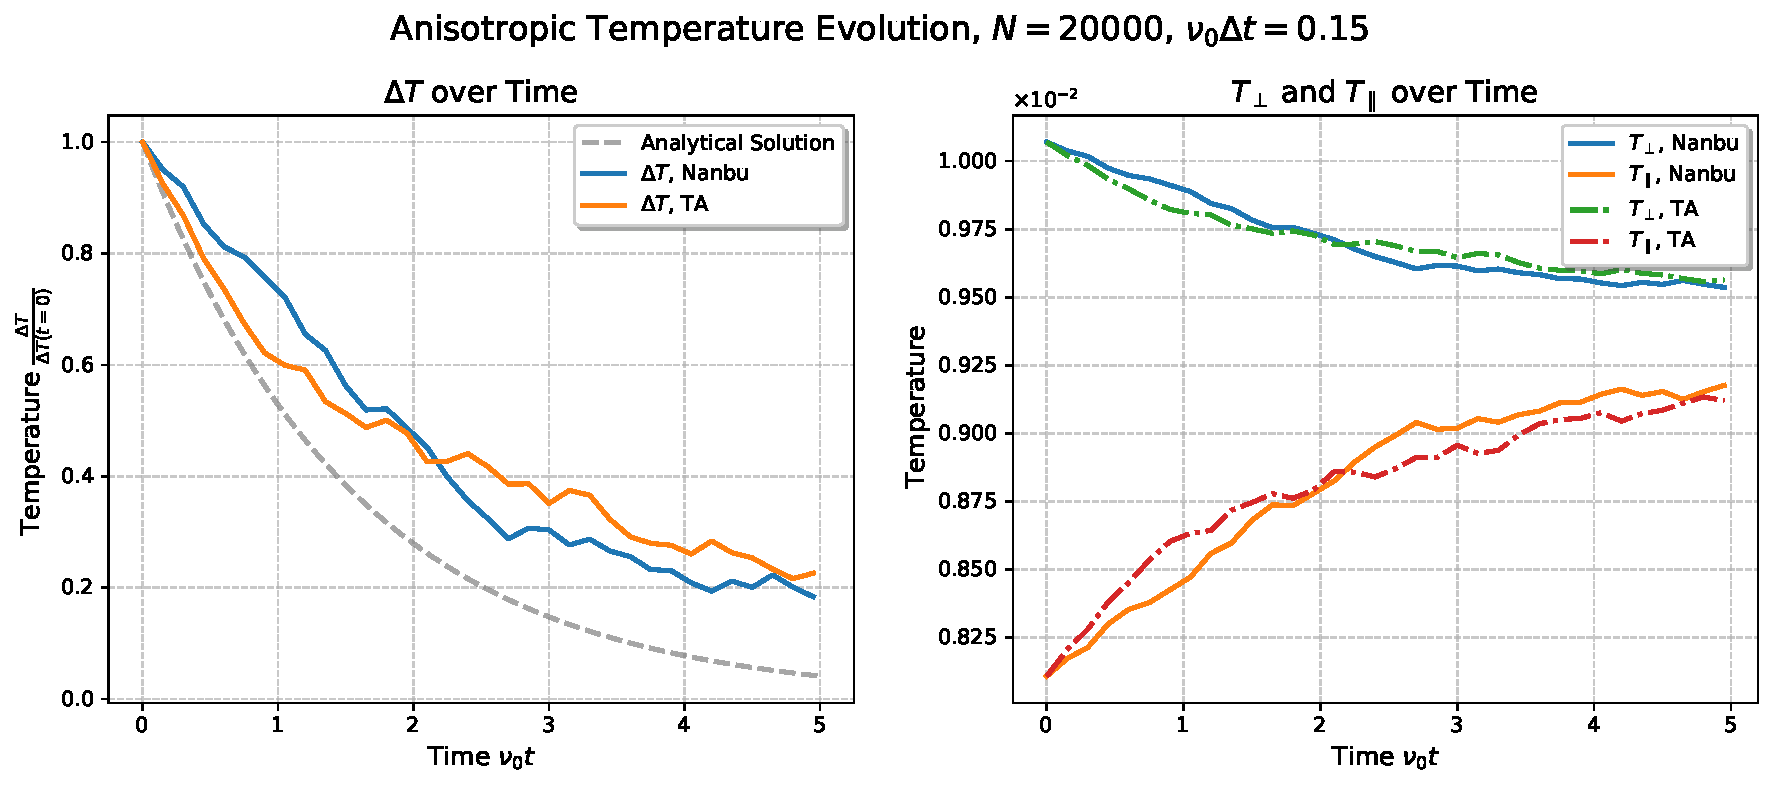
\includegraphics[width=\linewidth]{ressources/test1/anisotropic_T_example.pdf}
    \captionof{figure}{Temperature evolution using two different algorithms. The left panel shows temperature change $\Delta T = T_\perp-T_\parallel$ over time. The dashed line represents the analytical solution \eqref{eq:methodology:trubnikov_analytical_sol}. The right panel displays the temperature components for each method. The simulation uses $20000$ particles, a normalized final time of $\nu_0t = 5.0$, and a normalized time step size of $\nu_0\Delta t = 0.15$. Collision computation times were $0.18\,\si{\second}$ for Nanbu and $0.11\,\si{\second}$ for TA.}\label{img:test1:anisotropic_T_example}
    \vspace{5pt}
\end{minipage}
As expected, we see that the initial temperature components are correct up to slight statistical fluctuations. More important, we see that both methods methods result in similar behaviour, were the temperatures seem to get closer to a common value. 

However, it also becomes apparent that $N$ is by far not big enough to mitigate fluctuations. Because of that, the following analysis will include many realizations of every simulation. That way, we can also look at the ``uncertainty'' of each plot. 

\textbf{Different time step sizes.} The next part investigates the dependence of $\Delta T$ on $\nu_0\Delta t$ for different values. Each simulation is done using $2000$ realizations and $N=3200$ particles. The result is shown in figure \ref{img:test1:temperature_diff_dT_combined_shaded}. \\
\begin{minipage}[h]{\linewidth}
    \vspace{5pt}
    \centering
    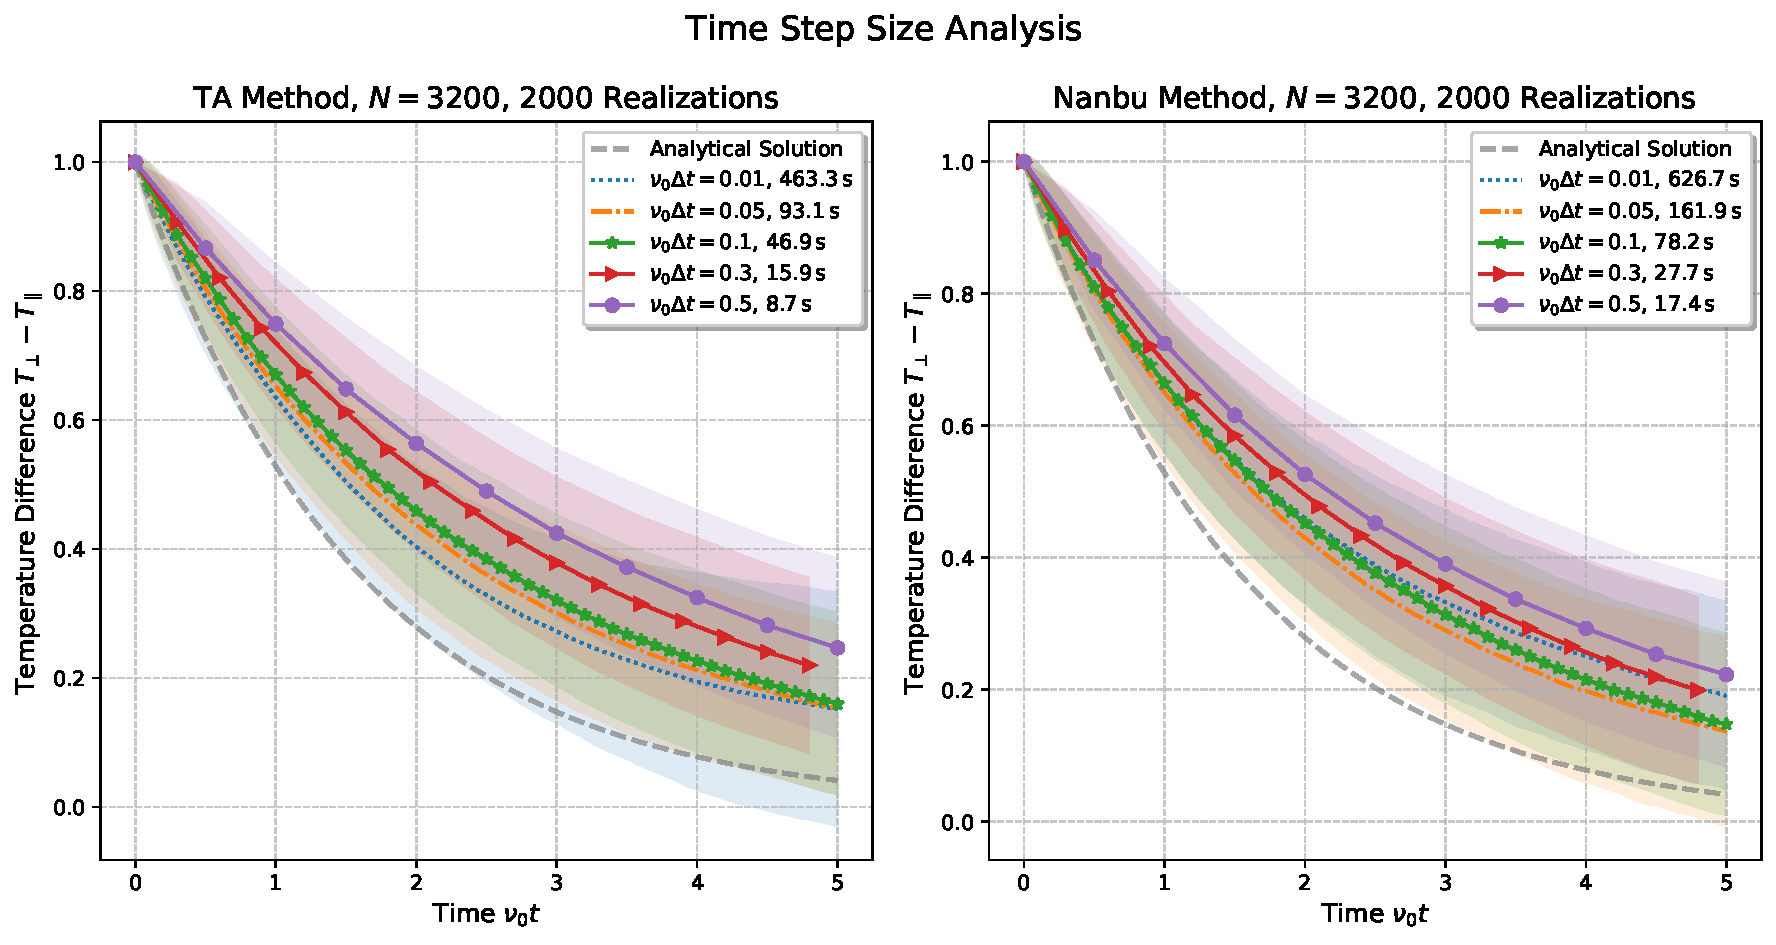
\includegraphics[width=\linewidth]{ressources/test1/temperature_diff_dT_combined_shaded.pdf}
    \captionof{figure}{Temperature evolution for Nanbu's and TA's method for different time step sizes. The simulation uses $3200$ particles and 2000 different realizations. The shaded region is the standard deviation of the realizations, the graph itself represents the mean. The time in the label denotes the overall computation time for the respective collision steps.}\label{img:test1:temperature_diff_dT_combined_shaded}
    \vspace{5pt}
\end{minipage}
The result shows two thing. First that the graph seems to converge to some value that is well above the analytical solution and second that smaller step size leads to better accuracy. The first effect is also observable in \cite[4313--4314]{Wang2008}. Here, the analytical solution seems to be around $\approx 0.3$ at $\nu_0t = 5$, while all simulations end up well above $0.4$. The paper does not mention it at all, but solves this discrepancy by comparing to a very fine calculated solution instead of the analytical graph. For this reason, the subsequent error analysis will be carried out in the same way by comparing to the $\nu_0\Delta t = 0.01$ solution.

Interestingly, the \textsc{Nanbu} method seems to converge only up to a specific very small value of $\nu_0\Delta t$ (see blue dotted line). This effect is not representative for this method, but rather shows a computational limitation. According to \cite[4645]{Nanbu1997}, the $A$ value used to sample the collision angle can be approximated by $A = s^{-1}$ for small $s$. If the time step size is too small, $A$ becomes very large, which in turn can lead to an overflow in the calculation of the angle $\cos \chi$. As soon as this happens, the algorithm catches that and puts $\Delta \mathbf{v} = 0$ (since $\lim_{A \rightarrow \infty} \cos\chi = 1$). However, this might lead to some inaccuracy, since many collisions are missing, even though their effect might be small and the relaxation becomes noticably slower.

\textbf{Different number of particles.} The same experiment as before can be run using $\nu_0\Delta t = 0.2$, $2000$ realizations and different number of particles. The result can be seen in figure \ref{img:test1:temperature_diff_N_combined_shaded}. \\
\begin{minipage}[h]{\linewidth}
    \vspace{5pt}
    \centering
    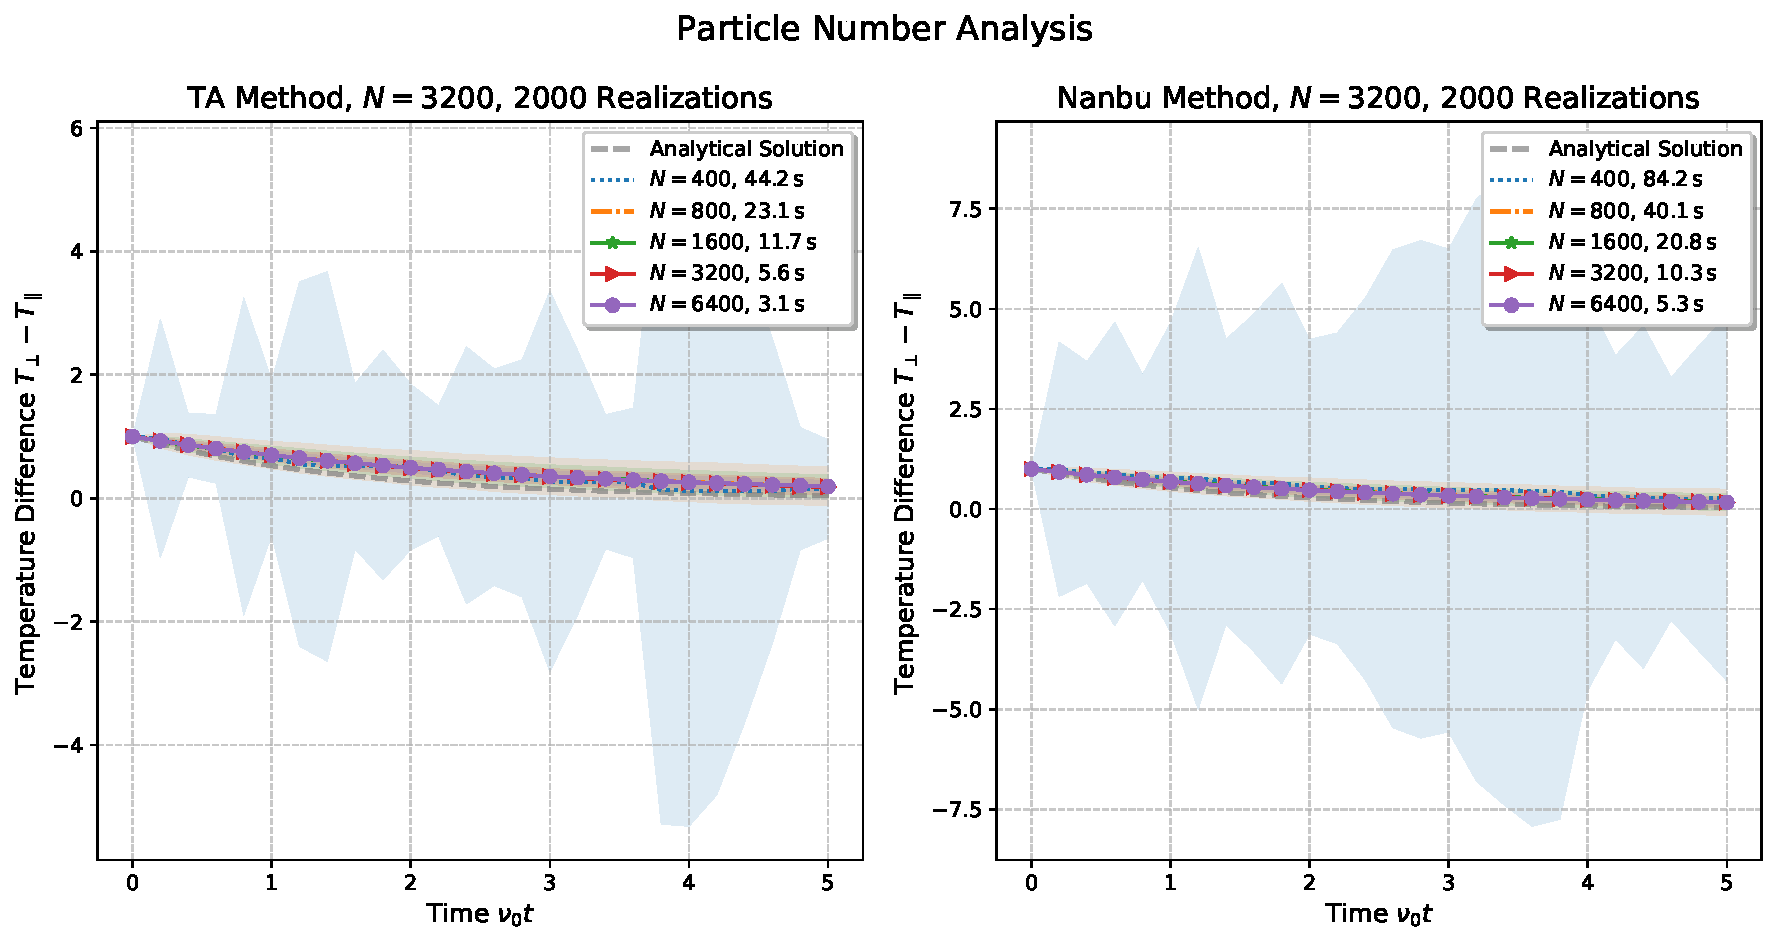
\includegraphics[width=\linewidth]{ressources/test1/temperature_diff_N_combined_shaded.pdf}
    \captionof{figure}{Temperature evolution for Nanbu's and TA's method for different number of particles. The simulation uses $\nu_0\Delta t = 0.2$ and $2000$ realizations each. The shaded region is the standard deviation of the realizations, the graph itself represents the mean. The time in the label denotes the overall computation time for the respective collision steps.}\label{img:test1:temperature_diff_N_combined_shaded}
    \vspace{5pt}
\end{minipage}
The most notable observation is that the shaded uncertainty is very large for a small number of particles. If we remove it, we get figure \ref{img:test1:temperature_diff_N_combined}. \\
\begin{minipage}[h]{\linewidth}
    \vspace{5pt}
    \centering
    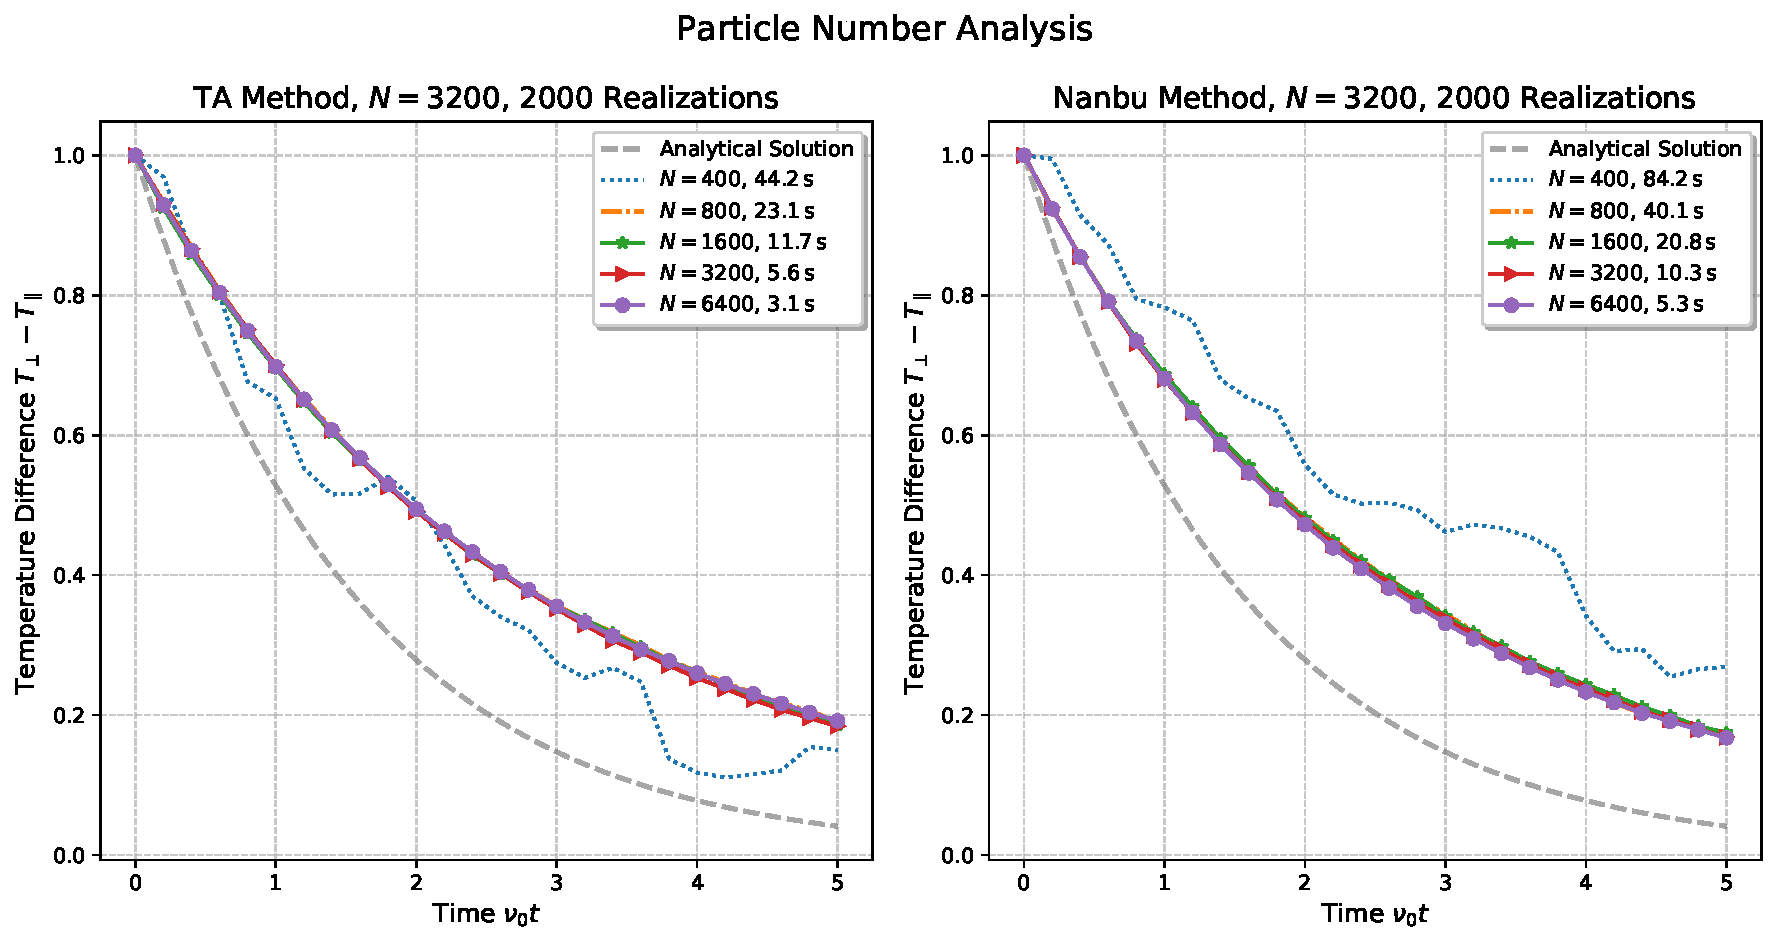
\includegraphics[width=\linewidth]{ressources/test1/temperature_diff_N_combined.pdf}
    \captionof{figure}{Temperature evolution for Nanbu's and TA's method for different number of particles without uncertainty. The parameters are the same as in figure \ref{img:test1:temperature_diff_N_combined_shaded}.}\label{img:test1:temperature_diff_N_combined}
    \vspace{5pt}
\end{minipage}
We see that the number of particles not seem to influence the accuracy of the solution, only the precision. This directly contradicts the expectation set by \cite[4317]{Wang2008}. The difference could be due to the fact that the density is set to be constant in figure \ref{img:test1:temperature_diff_N_combined_shaded}. \cite{Wang2008} does not mention anything about the density, so this is just a guess. However, it would make sense, since more particles mean a higher density and $\nu_0 \propto \sqrt{n}$. In that case, $\Delta t \propto \frac{\nu_0\Delta t}{\sqrt{n}}$ and the time step size decreases when the density is not controlled (the simulation domain remains the same). This then boils down to the exact same effect already observed in figure \ref{img:test1:temperature_diff_dT_combined_shaded}.

\textbf{Time step size error analysis.} Next, we can look at the convergence of the relaxation rate of the mean graph in figure \ref{img:test1:temperature_diff_dT_combined_shaded}. An linear function is fitted to the logarithm of the dataset and the rate is extracted from its slope. This process is repeated for every graph and the difference from the finest solution is plotted against $\nu_0 \Delta t$ in figure \ref{img:test1:relaxation_rate_convergence}. Note that the blue dotted line in figure \ref{img:test1:temperature_diff_dT_combined_shaded} of \textsc{Nanbu}'s method is not considered. \\
\begin{minipage}[h]{\linewidth}
    \vspace{5pt}
    \centering
    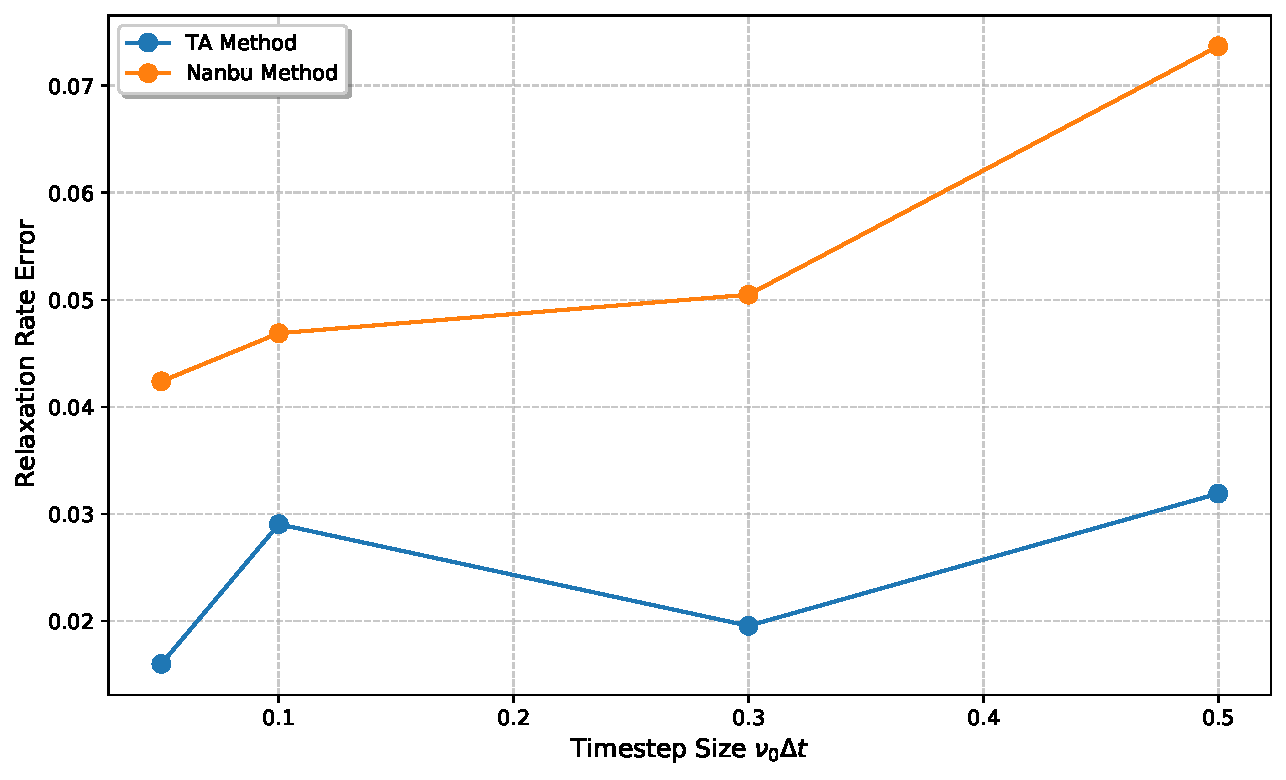
\includegraphics[width=0.75\linewidth]{ressources/test1/relaxation_rate_convergence.pdf}
    \captionof{figure}{Plot of the time step size $\nu_0 \Delta t$ against the error of the relaxation rate of the mean graphs in figure \ref{img:test1:temperature_diff_dT_combined_shaded}.}\label{img:test1:relaxation_rate_convergence}
    \vspace{5pt}
\end{minipage}
We see that the the error decreases for smaller time step sizes as expected. Fitting a linear function to these two graphs results in a slope of $0.18$ for \textsc{Takizuka} and \textsc{Abe}'s method and $0.20$ for \textsc{Nanbu}. These results are not too far off from \cite[4316]{Wang2008}, however, in order to get a real result, one would have to perform many more simulations than just four. The next part will also make it clear that the uncertainty of the relaxation rate is quite high\footnote{A hint might already be that the shaded regions in \ref{img:test1:temperature_diff_dT_combined_shaded} all contain all the other mean graphs as well.}. 

\textbf{Uncertainty analysis due to the number of particles.} Finally, the standard deviation at every point from the analysis in \ref{img:test1:temperature_diff_dT_combined_shaded} and \ref{img:test1:temperature_diff_N_combined_shaded} can be plotted. The graph is shown in figure \ref{img:test1:temperature_std_dt_comparison}. \\
\begin{minipage}[h]{\linewidth}
    \vspace{5pt}
    \centering
    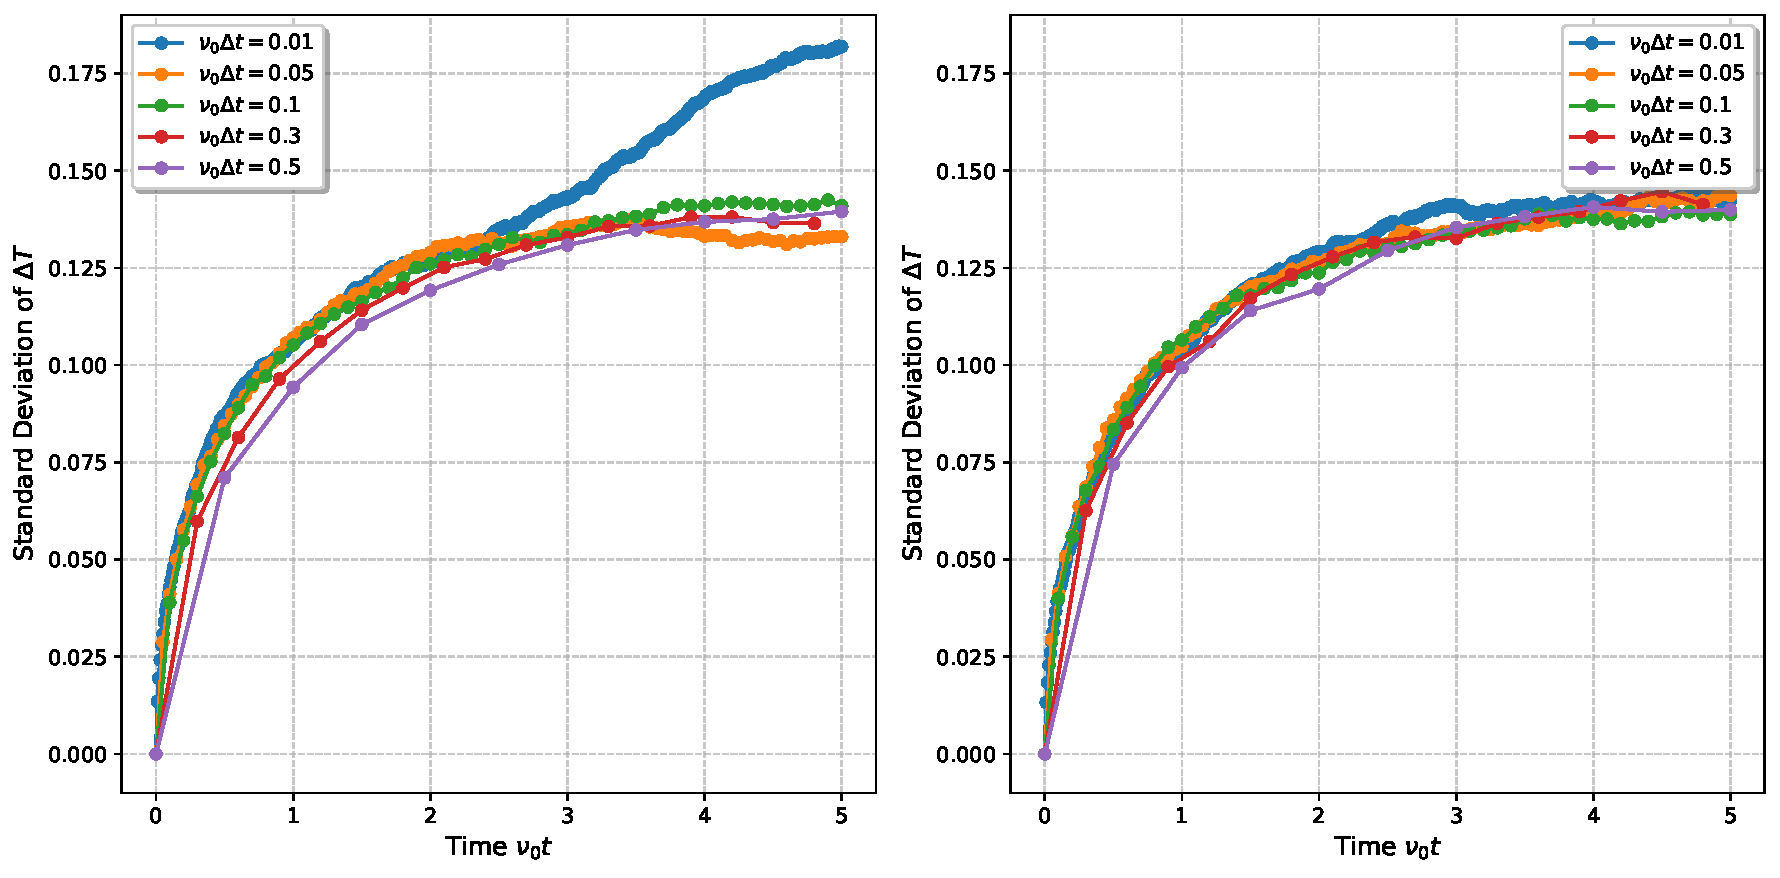
\includegraphics[width=\linewidth]{ressources/test1/temperature_std_dt_comparison.pdf}
    \captionof{figure}{Plot of the standard deviation of different realizations in figure \ref{img:test1:temperature_diff_dT_combined_shaded} for different time step sizes.}\label{img:test1:temperature_std_dt_comparison}
    \vspace{5pt}
\end{minipage}
You can see that the uncertainty for various values increases over time. The only outlier is $\nu_0 \Delta t = 0.01$ in TA's method. This might be a similar effect for very small step sizes as the same step size in \textsc{Nanbu}'s method, which -- as explained before -- converges slower due to missing collision computations. However, since this seems to be an outlier, it is not further investigated here.

The same can now also be done for the different number of particles and can be seen in figure \ref{img:test1:temperature_std_N_comparison}. Since the blue shaded area is much bigger and not smooth in figure \ref{img:test1:temperature_diff_N_combined_shaded}, we can conclude that $2000$ realizations are far too less to get a meaningful average. Because of that, we can ignore $N = 400$ in this plot. \\
\begin{minipage}[h]{\linewidth}
    \vspace{5pt}
    \centering
    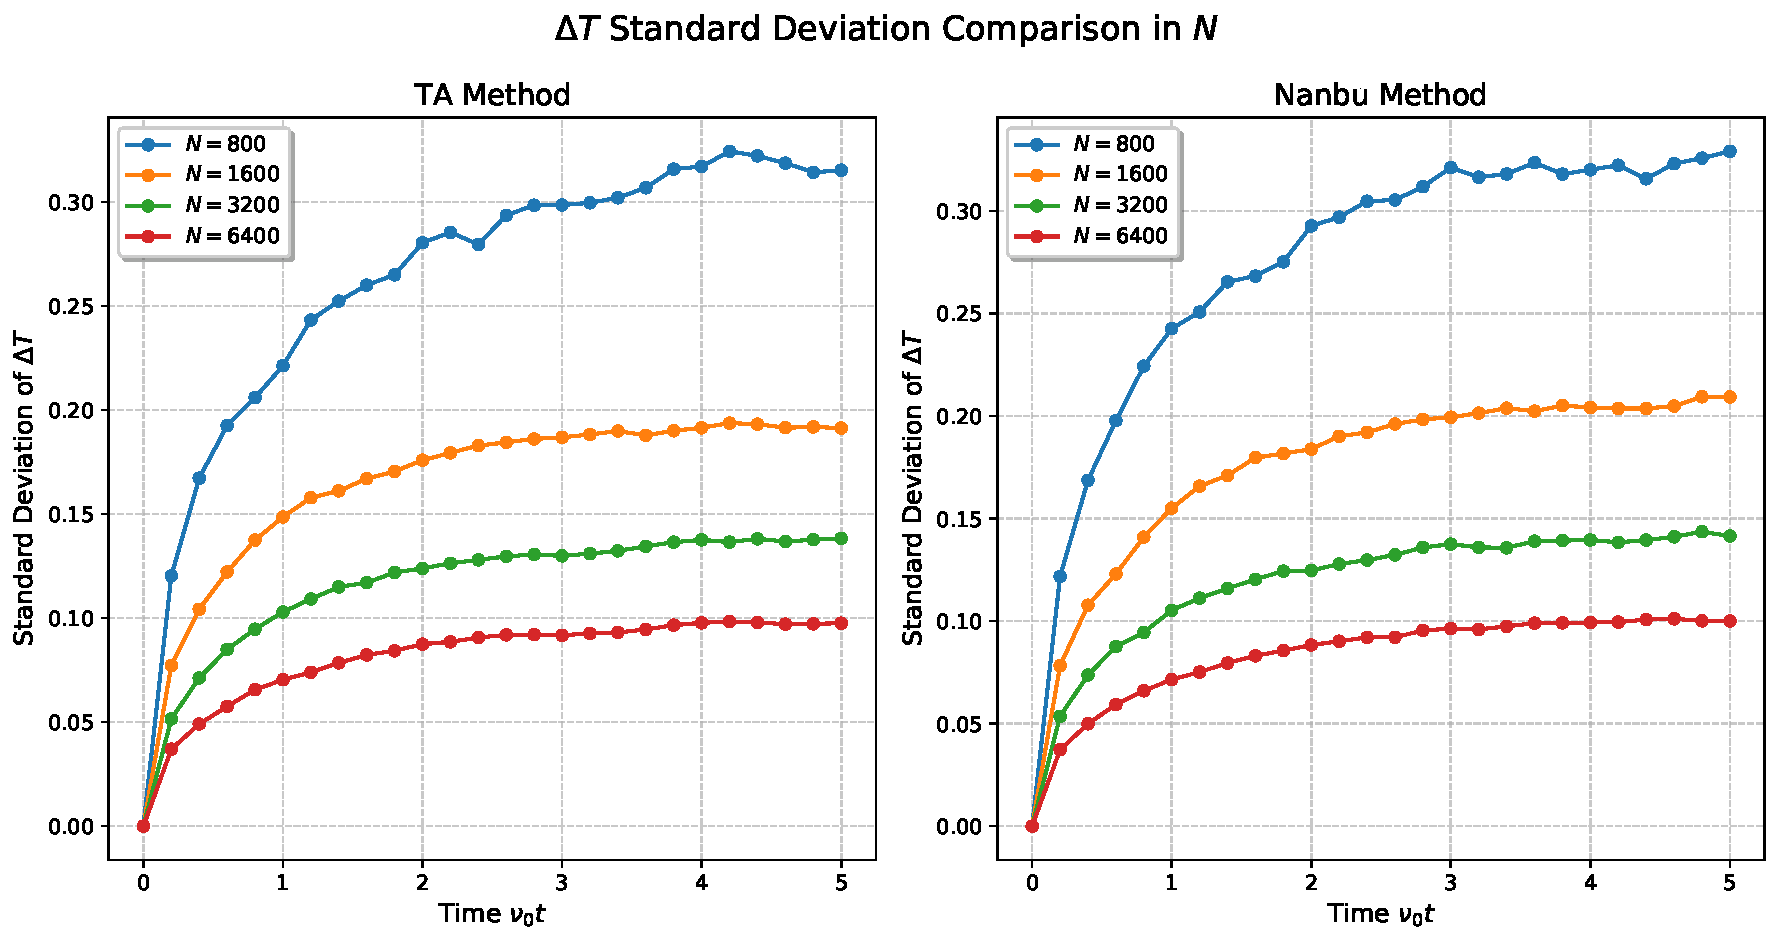
\includegraphics[width=\linewidth]{ressources/test1/temperature_std_N_comparison.pdf}
    \captionof{figure}{Plot of the standard deviation of different realizations in figure \ref{img:test1:temperature_diff_N_combined_shaded} for different number of particles.}\label{img:test1:temperature_std_N_comparison}
    \vspace{5pt}
\end{minipage}
This graph also very much looks like the expected result in \cite[4320]{Wang2008}. These two figure confirm that the uncertainty depends on the number of particles $N$, while the accuracy of the simulation mostly depends on the time step size $\nu_0 \Delta t$. 

% \subsection{Simple Relaxation Testcase}
% \subsection{Error in Time Step Size and $N$ Dependence}

% Use close-to-equilibrium testcase to show that the error to theoretical solution is dependent on the step size.
% Also shows that the algorithm actually works (validates my code...)
% TODO


\subsection{\textsc{Dirac} Distribution Relaxation Problem}

% Do an error vs cost comparison!
% Explain: does not work w/o field (since particles at dV=0 don't collide, do not get momentum)
Now that we established that both algorithms converge for small $\nu_0\Delta t$, we can consider a more complicated test case and possibly compare the results for both algorithms. Given that the simulation domain is a cube with periodic boundary conditions and the initial velocities are zero, we have an initial temperature $T_0 = 0$ and can calculate the expected equilibrium temperature $T_\mathrm{eq}$.

\textbf{Equilibrium temperature.} As mentioned in \ref{sec:methodology_and_testcases}, the positions are sampled with slight deviation from the center of origin to not run into the problem of infinite potential energy. The total potential energy of $N$ homogeneously distributed charged particles inside a cube of length $d_x$ can be calculated. With particle charge $q$, the potential energy between two particles separated by $r$ is given by $U = \frac{q^2}{4\pi r}$ (natural units). The average distance in a cube is given by $d_\mathrm{avg} \approx 0.66170d_x$ according to \cite{CubeLinePicking}. The number of unique possible pairs is $\mqty(N \\ 2) = \frac{N(N-1)}{2}$. Therefore, we get 
$$
U_0 = \frac{N(N-1) q^2}{8 \pi d_\mathrm{avg}} \approx 6.0131\cdot 10^{-2} \cdot \frac{N(N-1)}{d_x}
$$
using $q = 1$. If $L$ is the simulation domain length and we know that the system relaxes to a spatially homogeneous distribution, we can calculate the total potential energy that is converted to kinetic energy:
$$
E_\mathrm{kin,eq} = U_0 - U_\mathrm{eq} = 6.0131\cdot 10^{-2} \cdot N(N-1) \cdot \qty(\frac{1}{d_x} - \frac{1}{L}) .
$$
Using $E_\mathrm{kin} = \frac{m}{2} N \expval{\Delta \mathbf{v}^2}$ and $m=1$ and we get 
$$
T_\mathrm{eq} = \frac{2}{3 N} E_\mathrm{kin,eq} \approx 1.3421\cdot 10^{-2} \cdot (N-1) \cdot \qty(\frac{1}{d_x} - \frac{1}{L}) .
$$
%, where $\expval{\Delta \mathbf{v}^2} = \expval{v_x^2}+\expval{v_y^2}+\expval{v_z^2}$.
%Sampling $N$ particles in an initial cube of length $d_x$ gives the initial charge density $\rho_0 = \frac{Nq}{d_x^3}$, where $q$ is charge per particle. In natural units, the average

\textbf{Adaptive mesh sizing.} When the particles are homogeneously initialized inside a cube of size $d_x = \frac{L}{200}$ and a $64$ mesh grid, then all particles are inside on single cell drastically reducing the accuracy of the self consistent field solver. A possible solution is to implement an adaptive mesh grid size. This is done by computing the smallest and the biggest coordinate value for every particle and using these as new outer domain boundaries\footnote{Sidenote: There is a problem with this implementation. Since \texttt{AlpineManager.h} uses domain size variables to normalize the charge distribution, but the field solver objects uses the field layout as well as the mesh object. If the layout is changed without the mesh, we get badly scaled electric field values. However, adjusting the domain size variables also effects the application of the periodic boundary conditions. This results in a phenomenon where the particle domain becomes smaller and smaller, since the modified boundaries do not allow any expansion. The only way to fix this is to reset these boundary variables before calling the \texttt{.update()} routine. This fixes also potential charge conservation errors in multithreaded field solving.}. This operation is performed using a custom \texttt{MinMaxReducer} struct that can be called inside a \texttt{Kokkos::parallel\_reduce}. The outer boundaries are set before calling the field solver and reset after the gathering is done. 

We can first test this algorithm with a rather large $d_x = 0.1$ and get figure \ref{img:test2:T_E_V_comparison_adaptive_mesh_0.1}. \\
\begin{minipage}[h]{\linewidth}
    \vspace{5pt}
    \centering
    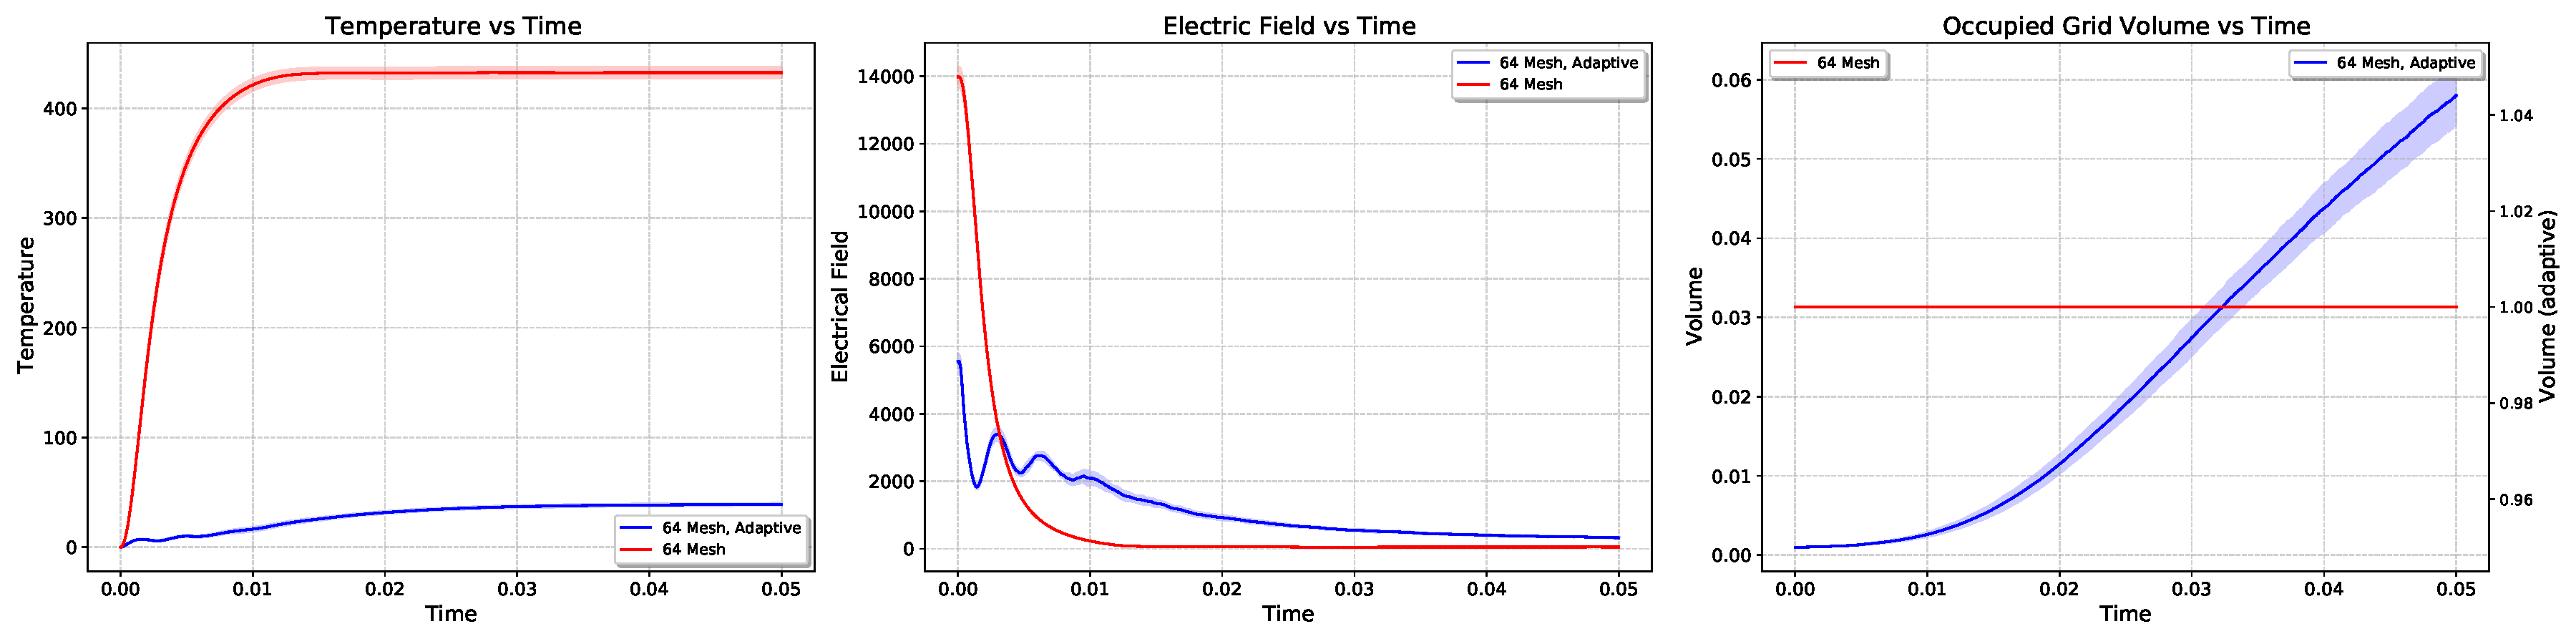
\includegraphics[width=\linewidth]{ressources/test2/T_E_V_comparison_adaptive_mesh_0.1.pdf}
    \captionof{figure}{Plot of the overall temperature, the mean field values of the self consistent field and the set domain volume against time. All simulations used a grid size of $64$, $1000$ particles, $d_x = 0.1$ and $500$ timesteps over 10 realizations each. Both plots were obtained using \textsc{Takizuka} and \textsc{Abe}'s collision algorithm. The shaded area represents the standard deviation over the realizations.}\label{img:test2:T_E_V_comparison_adaptive_mesh_0.1}
    \vspace{5pt}
\end{minipage}
There are simply not enough particles per cell to get an usable charge density for the solver. In that case, we see that the mean electric field in the beginning massively overshoots the blue (adaptive) value, which leads to a far accelerated expansion. Interestingly, if we use a much smaller $d_x = 0.005$, where -- without an adaptive grid -- all particles are within one cell, we get figure \ref{img:test2:T_E_V_comparison_adaptive_mesh_0.005}. \\
\begin{minipage}[h]{\linewidth}
    \vspace{5pt}
    \centering
    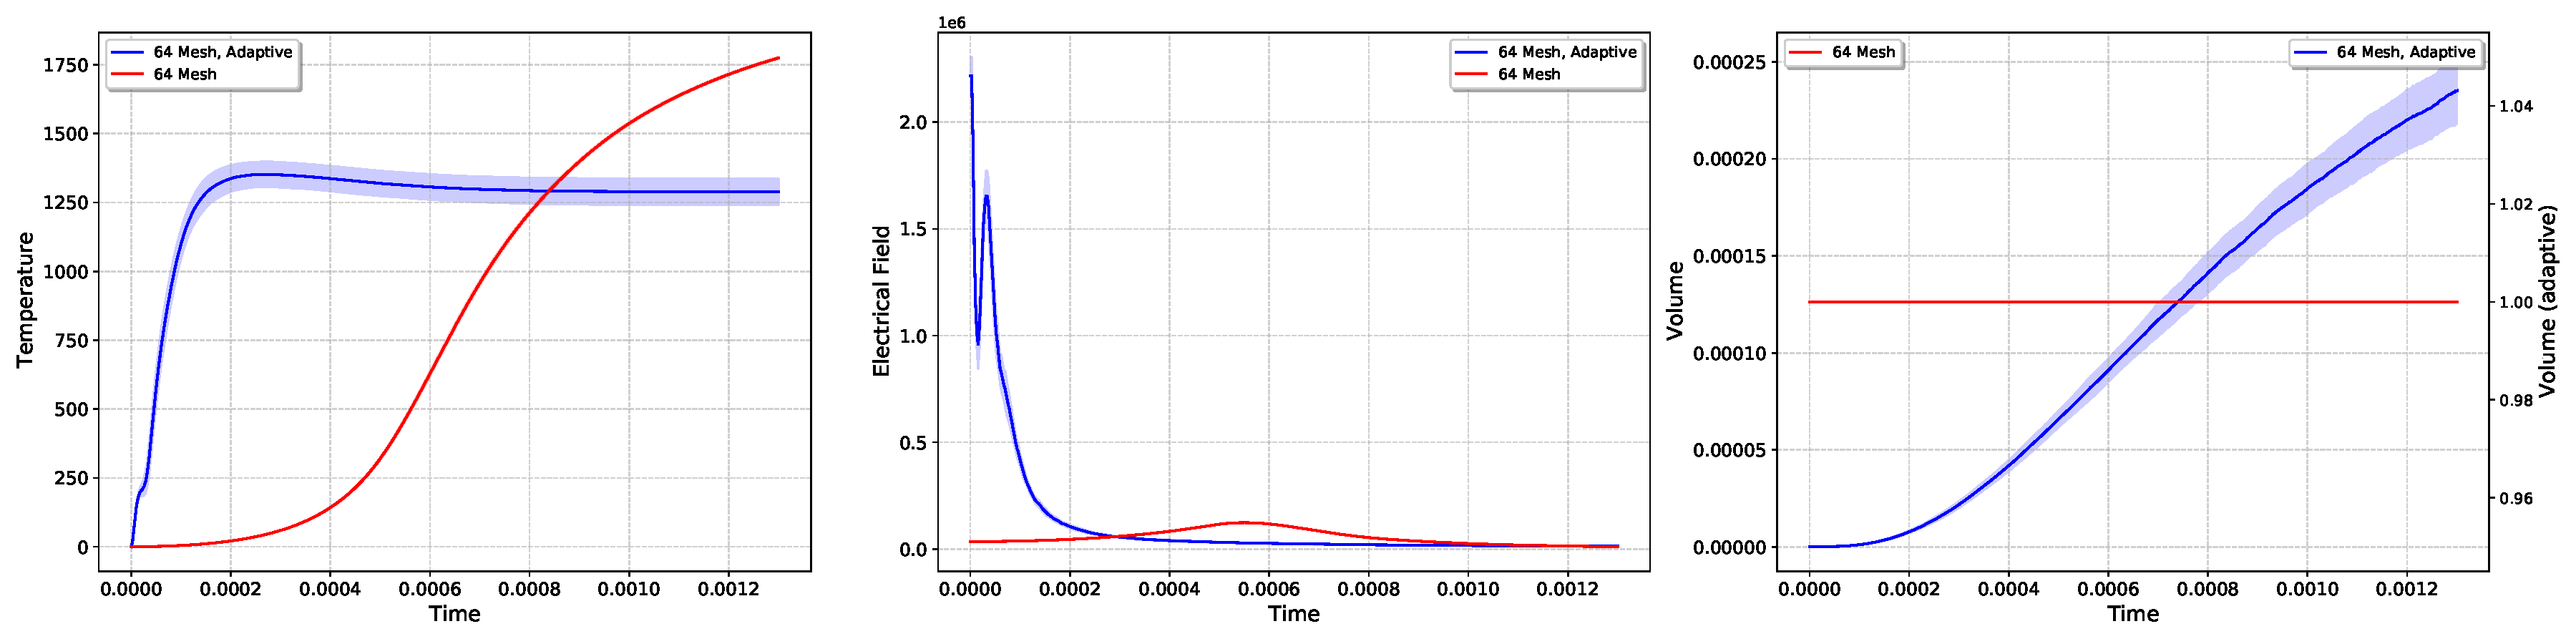
\includegraphics[width=\linewidth]{ressources/test2/T_E_V_comparison_adaptive_mesh_0.005.pdf}
    \captionof{figure}{Plot of the overall temperature, the mean field values of the self consistent field and the set domain volume against time, this time using $d_x = 0.005$. The rest matches figure \ref{img:test2:T_E_V_comparison_adaptive_mesh_0.1}.}\label{img:test2:T_E_V_comparison_adaptive_mesh_0.005}
    \vspace{5pt}
\end{minipage}
In this case, exactly the opposite happens and the solver massively underestimates the mean electric field. This is the more reasonable approach, since it actually uses a more ``delta like'' initial distribution. The reason for this behaviour is that underestimating the electric field leads to a smaller ``velocity burst'' that should rapidly expand the particle cloud in the beginning. Nevertheless, this $E$ spike appears a bit later (at around $0.0006$), which causes the temperature increase. After the cloud is big enough, where the occupied cloud volume is roughly $0.0002$, which corresponds to $d_x = \sqrt[3]{0.0002} \approx 0.05$, we see the same behaviour as in figure \ref{img:test2:T_E_V_comparison_adaptive_mesh_0.1}. $d_x$ then roughly matches the initial conditions of figure \ref{img:test2:T_E_V_comparison_adaptive_mesh_0.1} and the temperature begins to overestimating the adaptive solution, leading to a bigger relaxation temperature. Therefore, it makes sense to only use the adaptive algorithm from now on.

\textbf{Influence of Collisions.} Next, we can plot a test case to compare the effect of collisions. A run with no collisions, with \textsc{Nanbu} and with TA are plotted in figure \ref{img:test2:T_E_V_comparison_collision_algos_0.00005}. \\
\begin{minipage}[h]{\linewidth}
    \vspace{5pt}
    \centering
    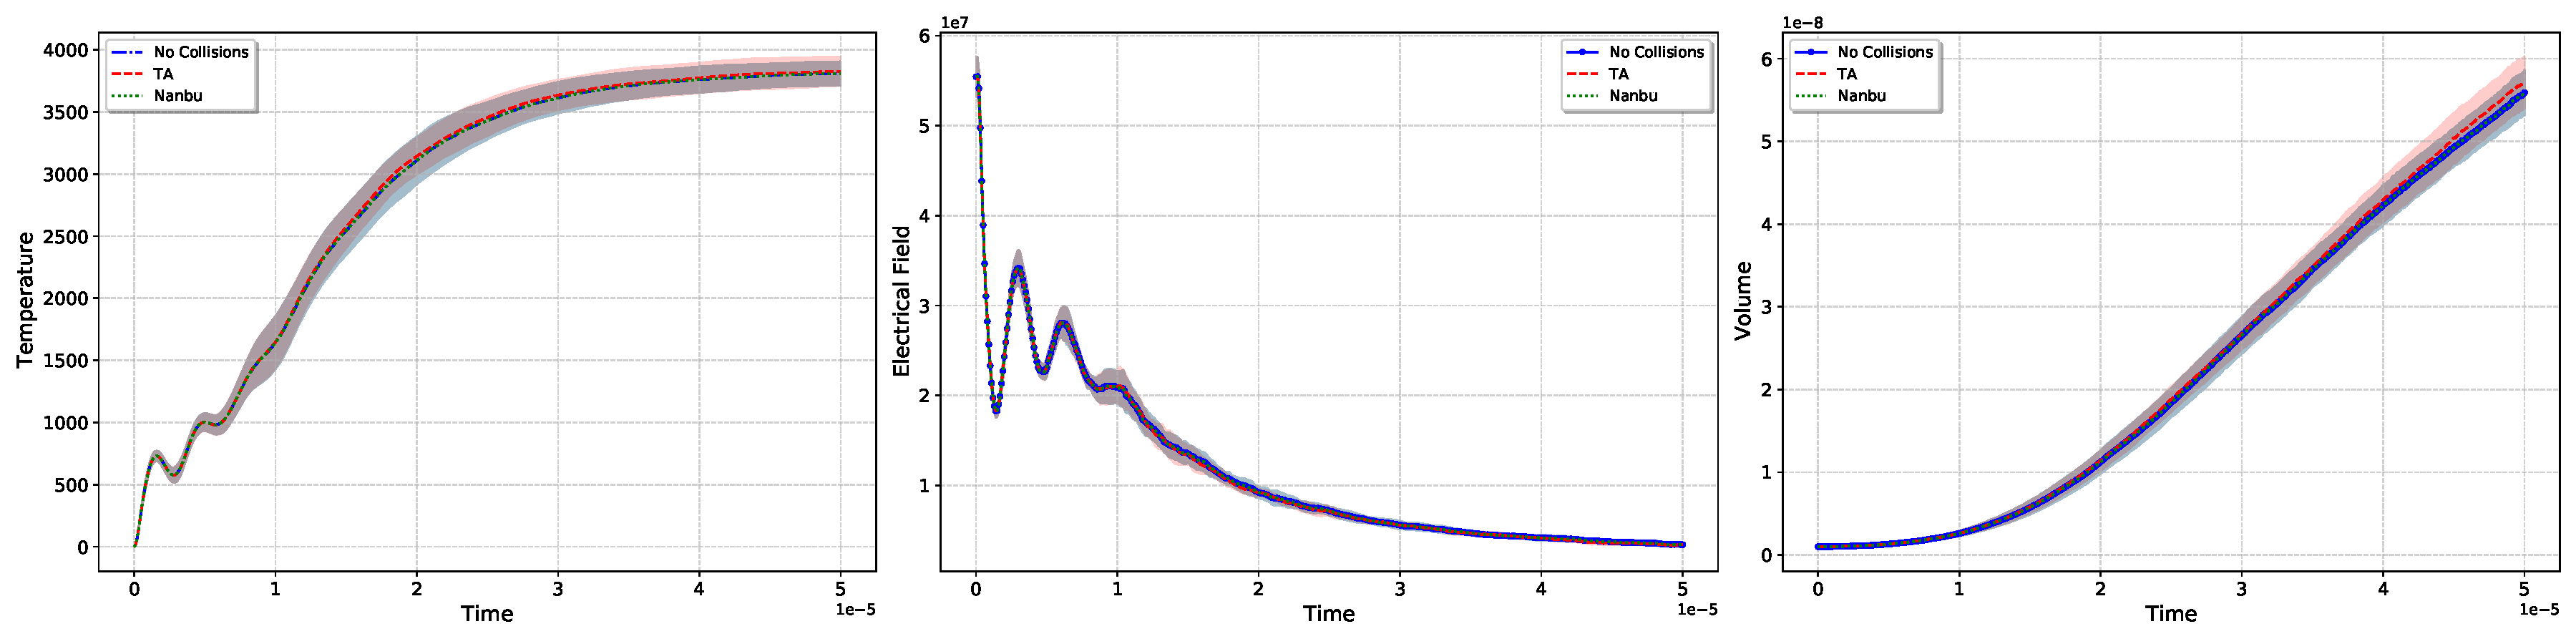
\includegraphics[width=\linewidth]{ressources/test2/T_E_V_comparison_collision_algos_0.00005.pdf}
    \captionof{figure}{Temperature, mean electric field and the set domain volume against time. Grid size $64$, $500$ time steps, $1000$ particles and $d_x = 0.001$ and 10 realizations each.}\label{img:test2:T_E_V_comparison_collision_algos_0.00005}
    \vspace{5pt}
\end{minipage}
At these conditions, there does not seem to be a big difference between the algorithms. The only notable difference is that TA is always slightly larger in all metrics than \textsc{Nanbu} and no collisions. The insignificance of the collisions comes from the fact that the in the beginning, the electric field is far too strong, which leads to high velocities and therefore suppresses the collision effect. The collisions can be observed only at either very large time steps, which in turn makes gives a large error due to velocities change from the electrical, or from low temperatures. To achieve that, we can either use less particles (reduces the electrical field) or use a rather large $d_x$. Doing both results in a slow relaxation, where the collisions become significant, see figure \ref{img:test2:T_E_V_comparison_collision_algos_5.0}. \\
\begin{minipage}[h]{\linewidth}
    \vspace{5pt}
    \centering
    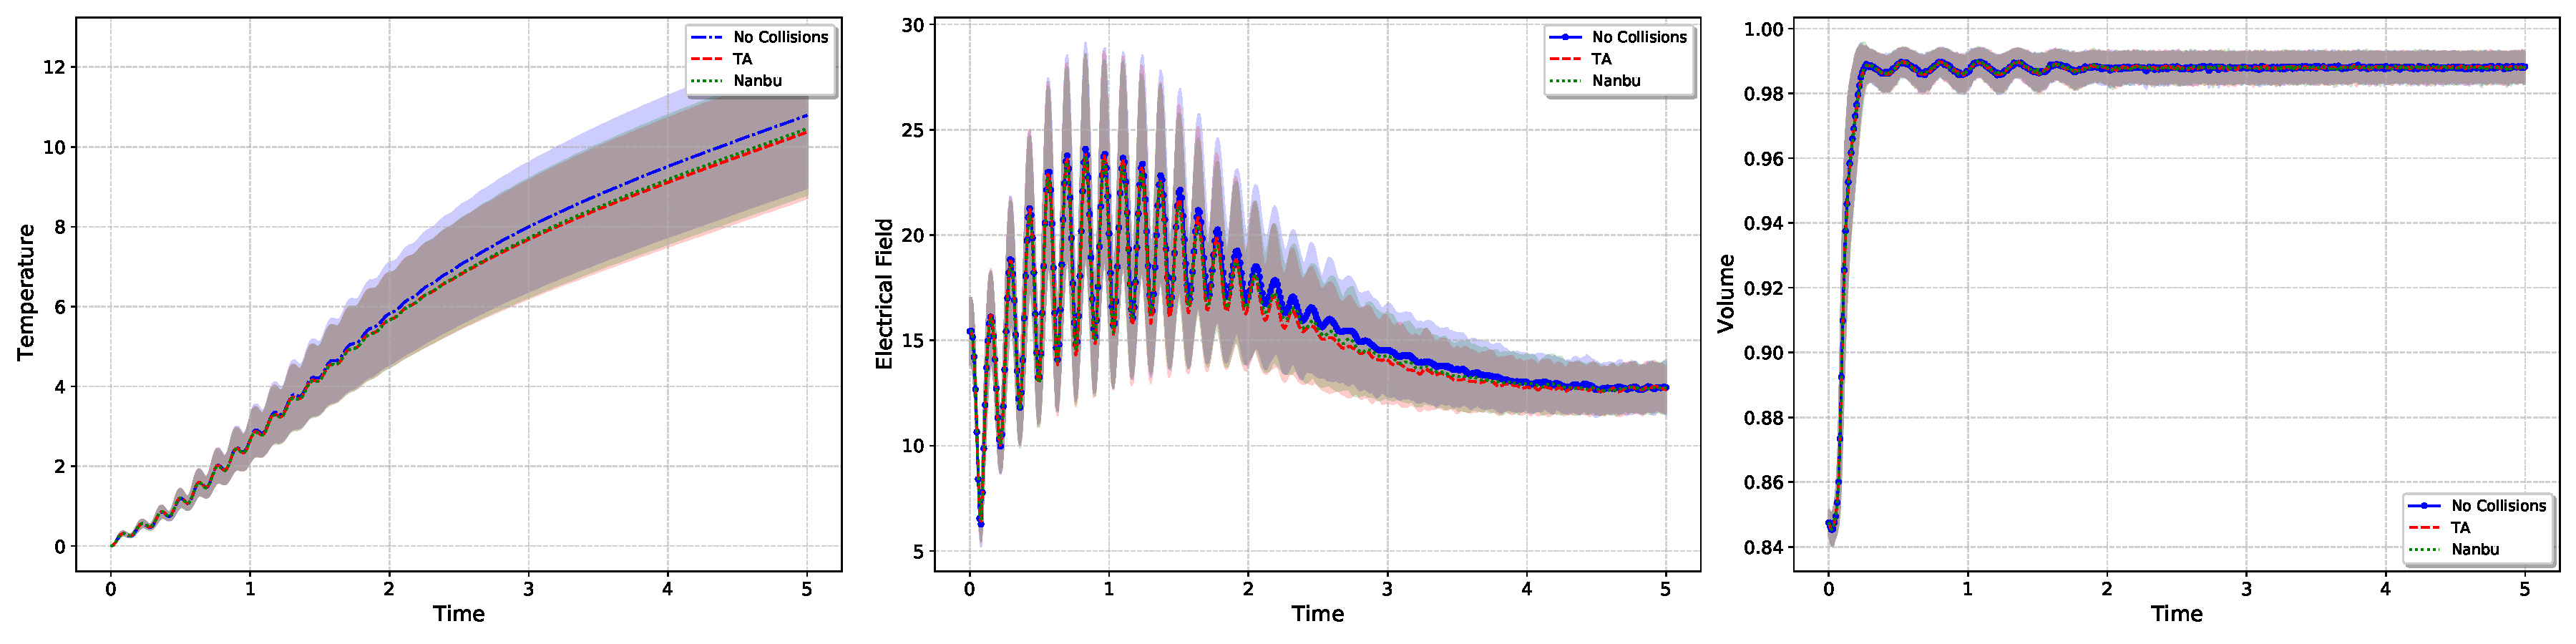
\includegraphics[width=\linewidth]{ressources/test2/T_E_V_comparison_collision_algos_5.0.pdf}
    \captionof{figure}{Temperature, mean electric field and the set domain volume against time. Grid size $8$, $500$ time steps, $500$ particles and $d_x = 0.95$ and $400$ realizations each.}\label{img:test2:T_E_V_comparison_collision_algos_5.0}
    \vspace{5pt}
\end{minipage}
We see that the collisions significantly -- even if the effect is small -- lower the relaxation temperature. However, there is no visible effect on the rate of expansion, meaning the graphs of the mesh volume are identical. This makes sense, since this should only be dependent on an overall change in velocity magnitude, which is driven by the electrical field.

%- Shows that accuracy and computation time analysis does not really make sense, since the collisions themselves are far from relevant for actual delta initial distribution cases (like \ref{img:test2:T_E_V_comparison_collision_algos_0.00005}) 
%- However, it might be more interesting to look at a few other factors like grid size and particle number --> do not use collisions, since for that regime, they are irrelevant 
The analysis of accuracy and computation time for these collision algorithms appears to be of limited relevance when considering actual delta initial distribution cases, as demonstrated in figure \ref{img:test2:T_E_V_comparison_collision_algos_0.00005}. Instead, it might be more fruitful to explore other aspects of the simulation, such as grid size and step size, while disregarding collisions altogether. 

\textbf{Influence of Mesh Grid Size.} To study the effect of grid size, we consider a simulation with $d_x = 0.001$ and focus on the initial rapid expansion. The result can be seen in figure \ref{img:test2:T_E_V_comparison_grid_sizing}. \\
\begin{minipage}[h]{\linewidth}
    \vspace{5pt}
    \centering
    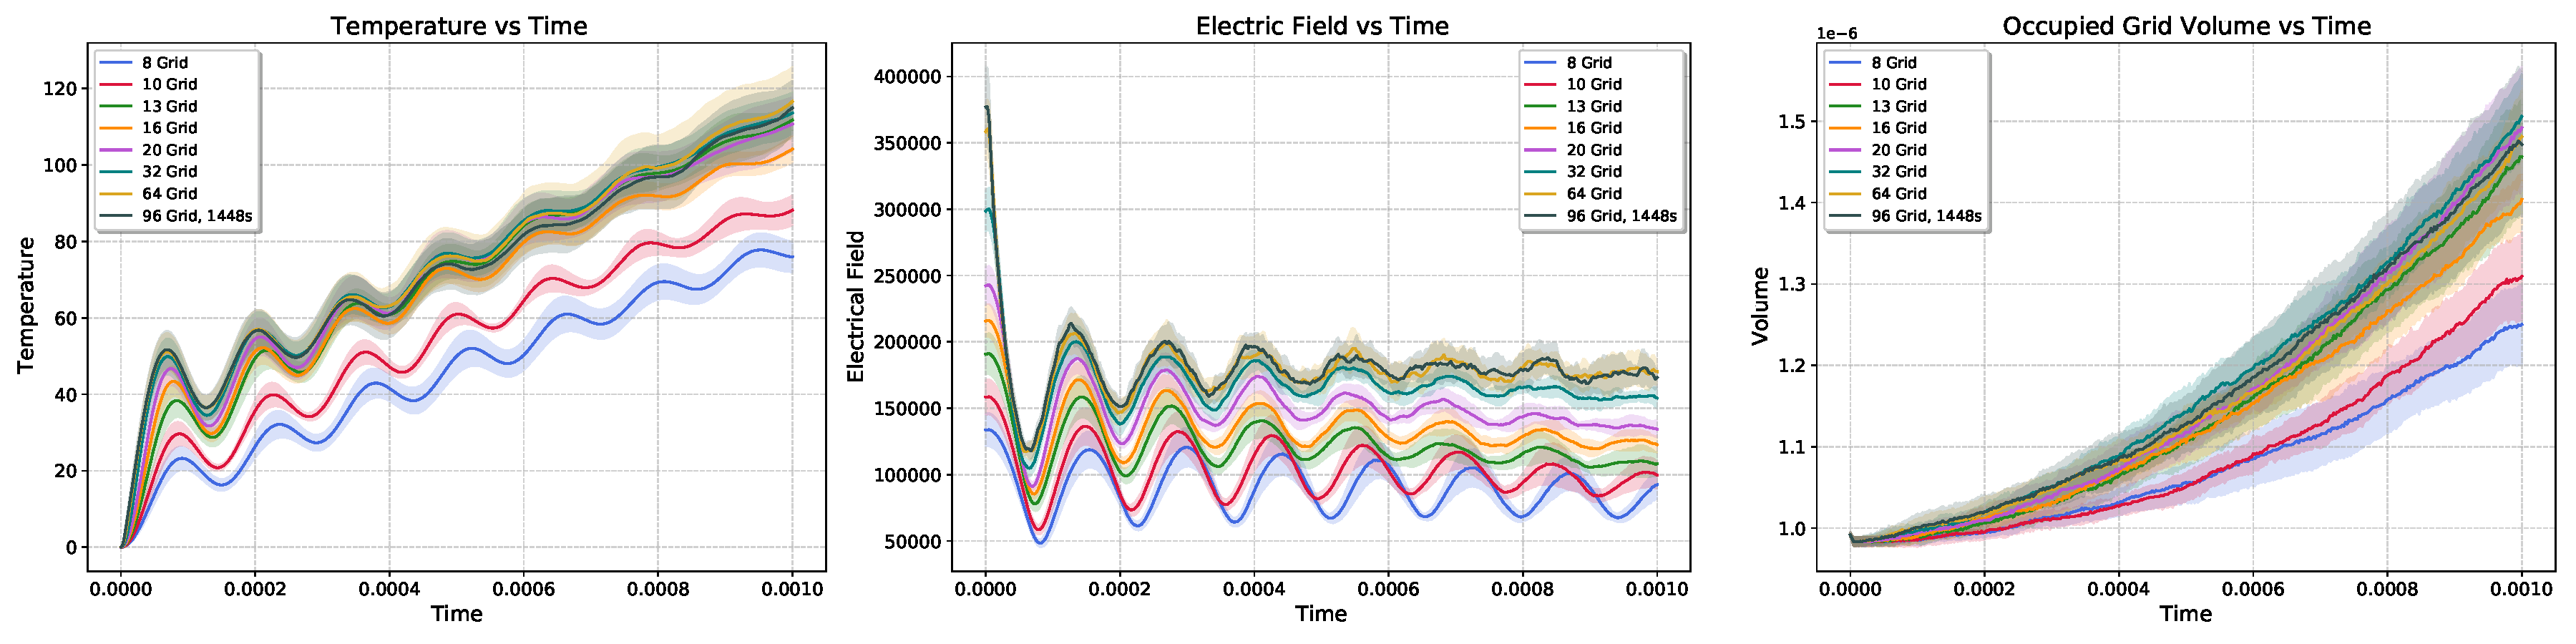
\includegraphics[width=\linewidth]{ressources/test2/T_E_V_comparison_grid_sizing.pdf}
    \captionof{figure}{Temperature, mean electric field and the set domain volume against time for different grid sizes. Each simulation uses $d_x = 0.01$, $N = 500$ particles, $400$ time steps and $10$ realizations. The shaded region is the standard deviation over these realizations.}\label{img:test2:T_E_V_comparison_grid_sizing}
    \vspace{5pt}
\end{minipage}
Generally, one can observe that the mean electric field values increase with the grid size. The reason for that is likely that there are not enough particles, which leads to possibly unoccupied cells. This also becomes apparent for after some time for grids with size over $20$, since the line of the electrical field is not smooth anymore and the standard deviation increases. 

As discussed before, the higher field values lead to higher velocities and therefore faster temperature increase and faster space expansion. Interestingly, there does not seem to be much of an accuracy increase after grid size $32$ in terms of temperature. A possible explanation is the overall linear upwards trend of the temperature. The overall increase in kinetic energy (which comes from the potential energy of the self consistent electrical field) overshadows the small accuracy differences that are still visible at $t \approx 0.0001$.

% which seems to happen because of energy conservation issues coming from the field. If the time step is too big in comparison to the field value, the velocity magnitudes overshoot the real value. The simulation technically uses a leapfrog step, which shoud be symplectic. But it is possible that 

\textbf{Influence of Step Size.} With the same simulation parameters as before, we get figure \ref{img:test2:T_E_V_comparison_timestepsize}. \\
\begin{minipage}[h]{\linewidth}
    \vspace{5pt}
    \centering
    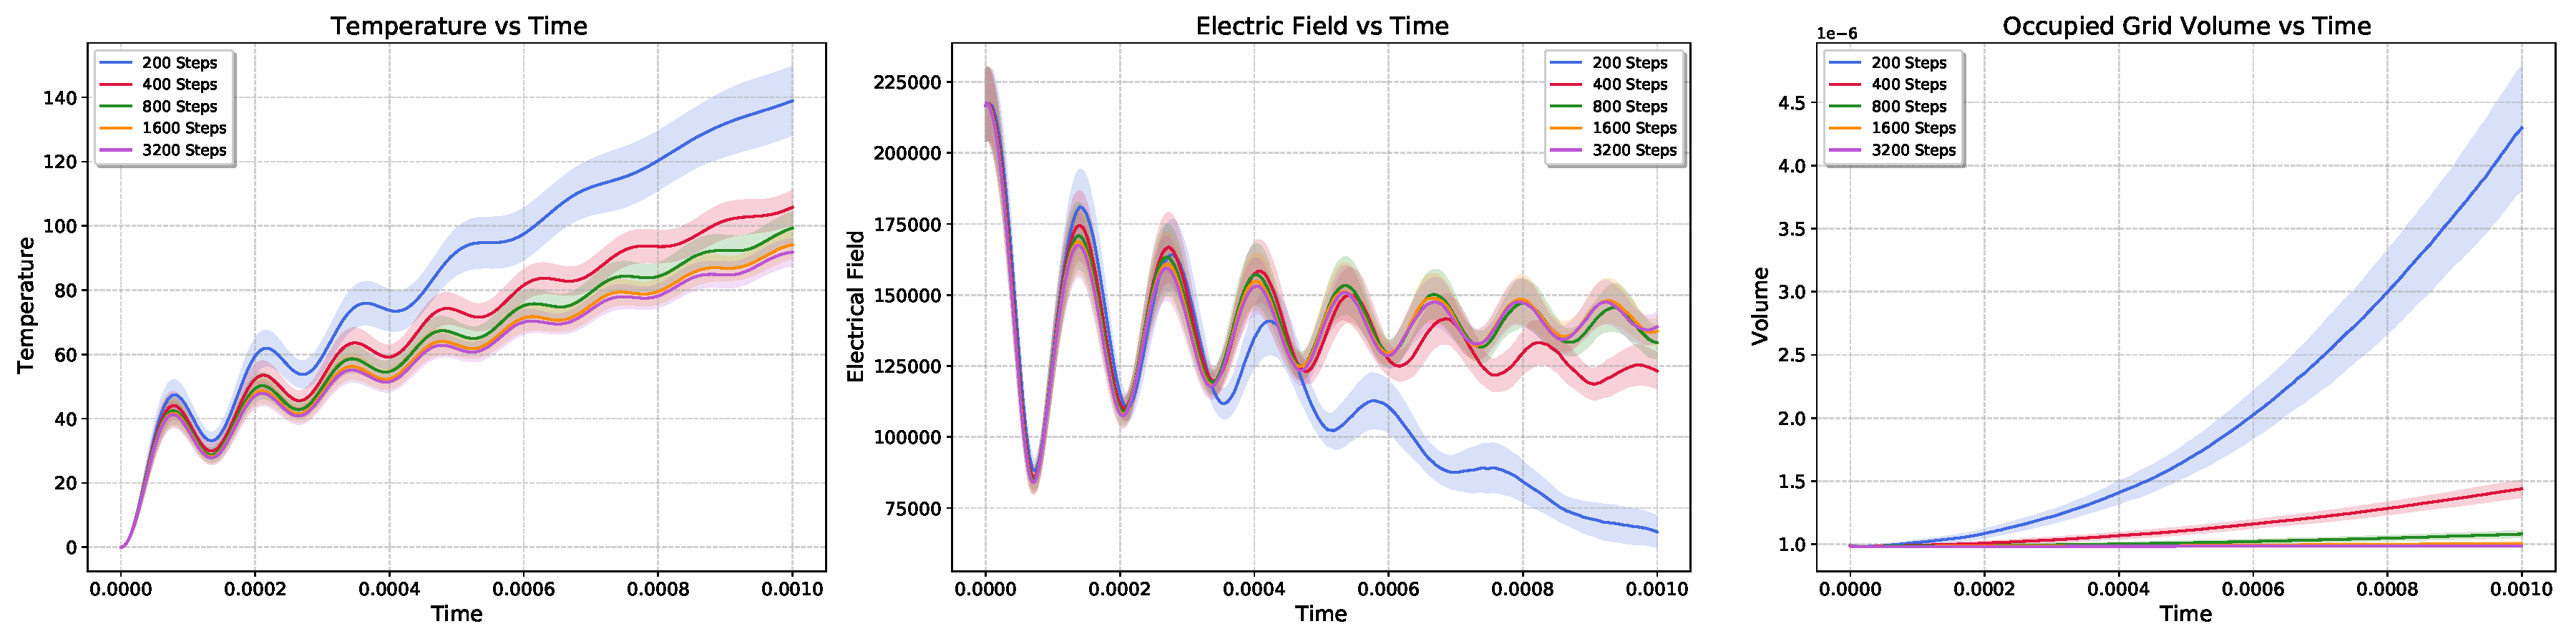
\includegraphics[width=\linewidth]{ressources/test2/T_E_V_comparison_timestepsize.pdf}
    \captionof{figure}{Temperature, mean electric field and the set domain volume against time for different numbers of time steps. Each simulation uses $d_x = 0.01$, $N = 500$ particles, a grid size of $16$ and $100$ realizations. The shaded region is the standard deviation over these realizations.}\label{img:test2:T_E_V_comparison_timestepsize}
    \vspace{5pt}
\end{minipage}
The number of time steps (and therefore the time step size)  directly influences the accuracy of the simulation. Even though, the temperature or electric field differences are not that far off for other time step sizes, the occupied grid volume seems to be affected a lot. This means that the particle cloud expands much faster for bigger step sizes, which might even lead to energy conservation issues when simulating for longer. 

Finally, we can compare the graphs against the ``fine solution'' with $3200$ time steps and see how fast it converges (figure \ref{img:test2:T_E_V_comparison_timestepsize_errors}). \\
\begin{minipage}[h]{\linewidth}
    \vspace{5pt}
    \centering
    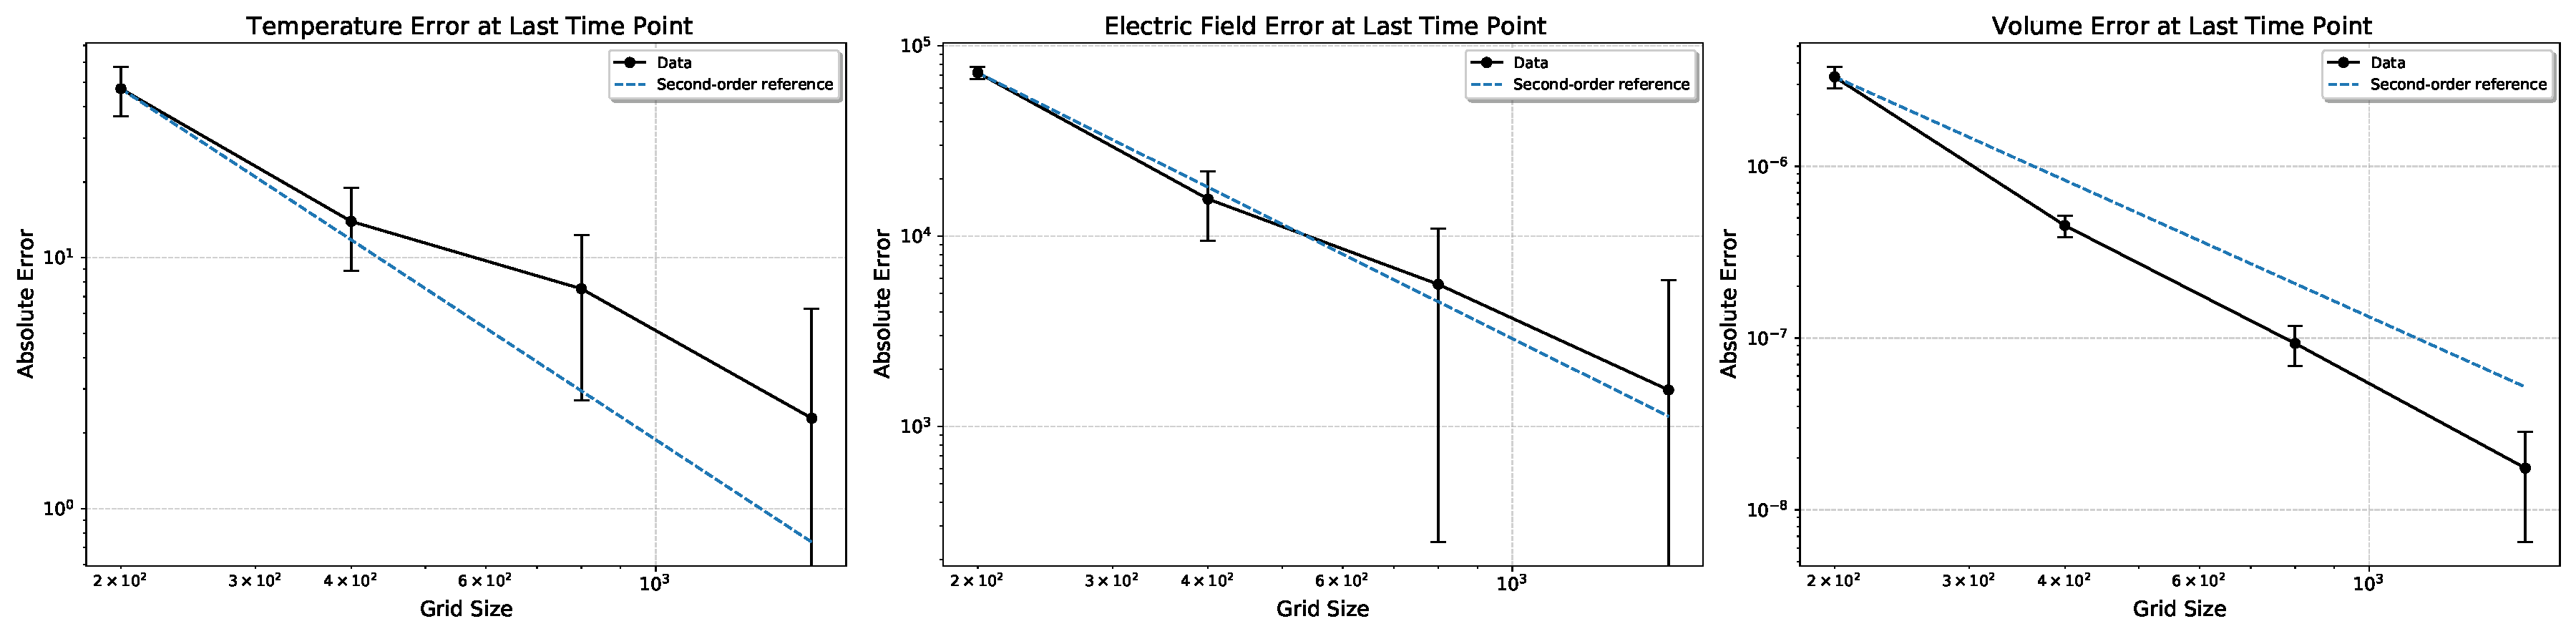
\includegraphics[width=\linewidth]{ressources/test2/T_E_V_comparison_timestepsize_errors.pdf}
    \captionof{figure}{Error plot against number of time steps for the graphs in figure \ref{img:test2:T_E_V_comparison_timestepsize}.}\label{img:test2:T_E_V_comparison_timestepsize_errors}
    \vspace{5pt}
\end{minipage}
All of these metrics are quite close to a second order convergence. This is to be expected, since the algorithm uses a leapfrog step to advance particle velocity and position.

%- Conclusion: this test case was not suitable to compare takizuka abe and nanbu --> better would be the Trubnikov test \ref{sec:result:trubnikov}
%- Could see come convergence behaviour; still useful
%- Confirmed that the adaptive grid sizing is very useful for this kind of test.
In conclusion, this test case was not ideal for comparing the \textsc{Takizuka} \& \textsc{Abe} and \textsc{Nanbu} methods; a more appropriate scenario is still the \textsc{Trubnikov} test, as discussed in section \ref{sec:result:trubnikov}. Despite this limitation, some convergence behavior was observed, indicating that the results still hold value. Additionally, the findings confirmed the effectiveness of adaptive grid sizing, which proved to be particularly beneficial for this type of test. 
% Overall, while the comparison may not have been optimal, the insights gained contribute to our understanding of the methods involved.
% TODO
%0159 4000_Nanbu...: ./Nanbu delta 72 5 0.1 Nanbu 1000 0.005 4000 false true true --info 10
%0159 4000_TakAbe...: ./Nanbu delta 72 5 0.1 TakAbe 1000 0.005 4000 false true true --info 10
%1239 4000_Nanbu_...: ./Nanbu delta 32 5 0.1 Nanbu 1000 0.005 4000 false true true --info 10cd


\subsection{Disorder Induced Heating of a Cold Sphere}\label{sec:result:coldSphere}

% Do the same as for Dirac distribution...
% This test case is designed to simulate a disorder-induced heating processes of a particle sphere. We use a $25 \si{\femto\coulomb}$ spherical electron bunch ($156055$ particles) with zero initial momentum spread. The initial coordinates of the electron are randomly distributed within a spherical area of radius $R$. The electron beam is stationary and constrained in the radial direction by a linear focusing force equal to and opposite to the repulsive force generated by the mean space charge field. These parameters are chosen to correspond to possible beam charges and densities near a photoelectron gun used for ultrafast electron diffraction according to \cite{mitchell2015parallel}.

% We calculate the time evolution of the normalized x-emittance as a key measure of beam quality. The emissivity formula is:
% \begin{equation}
%     \varepsilon_{x, \mathrm{rms}}=\sqrt{\left\langle x^2\right\rangle\left(\left\langle p^2\right\rangle\right)-(x p)^2},    
% \end{equation}
% where $\left\langle x^{2}\right\rangle$ and $\left\langle p_{x}^{2}\right\rangle$ represent the averages of $x^{2}$ and $p_{x}^{2}$, respectively. 

% Using $k_\mathrm{B}T \approx 7.69\,\si{\milli\electronvolt}$ to get a Debye length of approximately the gridsize for a $64^3$ grid and $L = 100 \,\si{\micro\metre}$, we get figure \ref{img:sphere:energy_spread} for the emittance plot. TODO: add derivation for this value \\
% \begin{minipage}[h]{\linewidth}
%     \vspace{5pt}
%     \centering
%     \includegraphics[width=0.7\linewidth]{ressources/xemittance_plot.pdf}
%     \captionof{figure}{TODO: add caption}\label{img:sphere:energy_spread}
%     \vspace{5pt}
% \end{minipage}
% Looking at the energy, we get \ref{img:sphere:energy_spread}. \\
% \begin{minipage}[h]{\linewidth}
%     \vspace{5pt}
%     \centering
%     \includegraphics[width=0.7\linewidth]{ressources/energy_plot.pdf}
%     \captionof{figure}{TODO: add caption}\label{img:sphere:energy_spread}
%     \vspace{5pt}
% \end{minipage}
% TODO: problem: no collision effects visible, need to modify initial velocites (?) s.t. they matter!

% picture analyse points: 

% After a quarter plasma cycle, the electrons' initial positional disorder is converted into momentum disorder through a disorder-induced heating process. The beam will reach a final equilibrium temperature $T_\mathrm{eq}$, which is approximately equal to the plasma coupling parameter.
Using the parameters outlined in \ref{sec:methodology_and_testcases}, we want to replicate the results from \cite[595]{Mitchell2015}. The paper uses a cutoff radius up to which ``collisions'' are relevant. This parameter does not exist for our algorithms. However, by choosing different grid sizes, we can effectively get a similar result, since only collisions in one mesh grid cell are considered. The result can be seen in figure \ref{img:test3:cold_sphere_grid_comparison}. \\
\begin{minipage}[h]{\linewidth}
    \vspace{5pt}
    \centering
    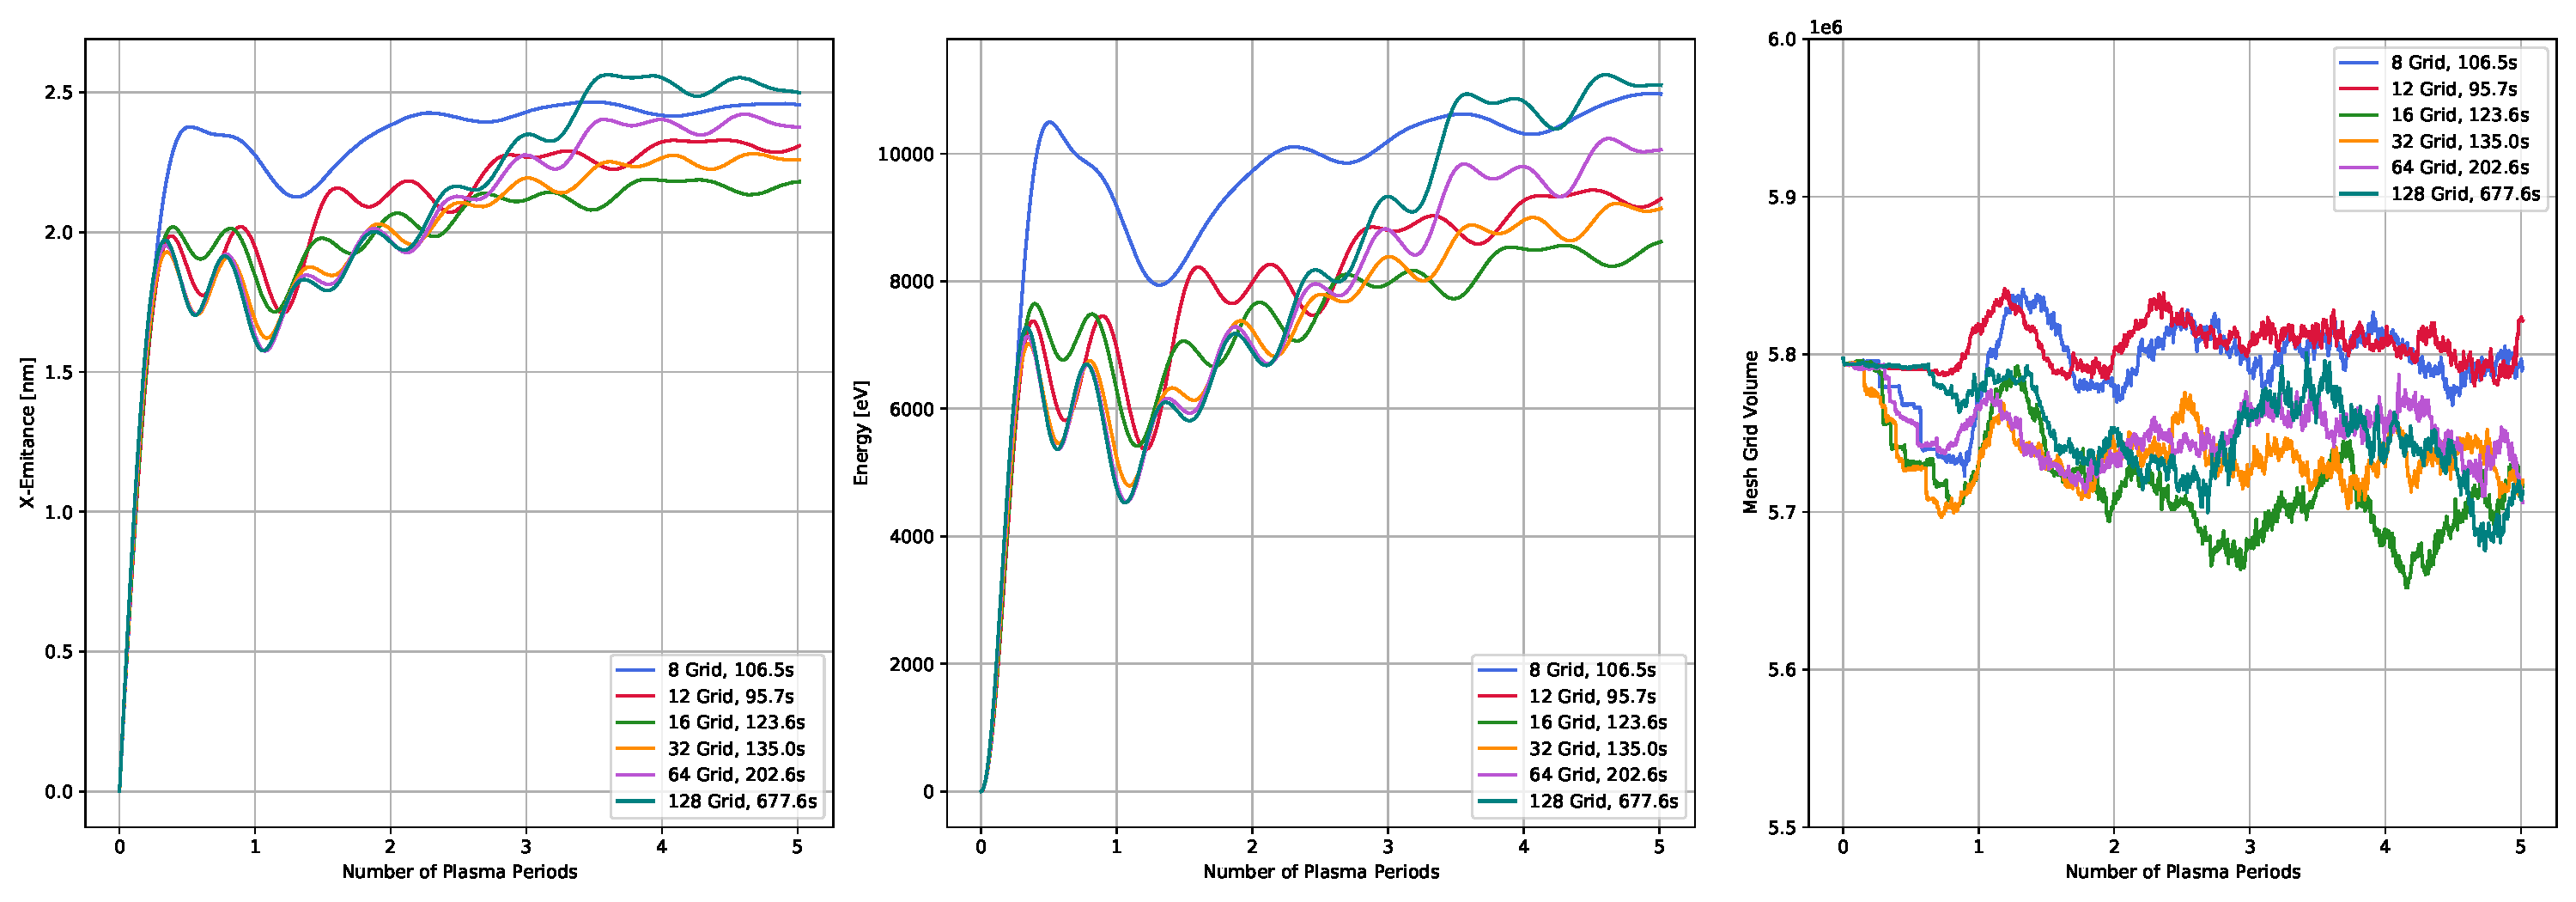
\includegraphics[width=\linewidth]{ressources/test3/cold_sphere_grid_comparison.pdf}
    \captionof{figure}{$x$-emittance, total energy and mesh grid volume against time for different mesh grid sizes. All simulations were done using only one realization with \textsc{Takizuka} and \textsc{Abe}'s collision algorithm.}\label{img:test3:cold_sphere_grid_comparison}
    \vspace{5pt}
\end{minipage}
As one can see, the confinement works well. However, it does not \textit{only} consist of the linear focusing force, but also of reflecting boundary conditions in a sphere of radius $R_0$. This was necessary, since otherwise the bunch would always expand if the force is slightly to small and shrink if it is too big (which causes the energy to spike).

Looking at the oscillations themselves, we can see that they appear to be of the expected result. A fast \textsc{Fourier} transform for the $64$-grid reveals that the most represented wave period are 
$$
2.16\cdot 10^{-11}\,\si{\second},
\qquad 6.49\cdot 10^{-11}\,\si{\second},
\qquad 3.24\cdot 10^{-11}\,\si{\second} .
$$
The average is roughly $4\cdot 10^{-11}\,\si{\second}$, when the theoretical result is $\approx 4.31\cdot 10^{-11}\,\si{\second}$. Even though the simulation does not look as clean as in \cite[595]{Mitchell2015}, it provides the correct result for the oscillation.

%Reasons why the simulation does not look as clean:
%- adaptive mesh sizing --> even a 32 has roughly the same density resolution as a 128 mesh without adaptive mesh
%- That's why the 8 grid is the only one that seems to be a bit off
%- Differences come mostly from collisions during the beginning
%    -> after certain time the velocities are to high
%    -> collisions become insignificant
%    -> only field solution is relevant after the initial burst
%    -> can see: solutions are very similar during the first oscillation period!
%- Why does it not look smooth? Scaling issue with the adaptive mesh size --> same parameters, but does not look as nice as previous result (see figure \ref{img:additional:disorder_heating_grid_comparison}), when the adaptive grid is not used 
%    -> previous result had constant grid size, which is why the 16 grid already ``diverges''
%    -> they had also the correct order of magnitude for the emittance --> confirms scaling issue
The simulation results appear less clean due to several factors related to adaptive mesh sizing. Notably, even a 32 mesh exhibits a density resolution comparable to that of a 128 mesh without an adaptive mesh, which is why only the 8-grid seems somewhat off in comparison. Discrepancies between each simulation primarily arise from collisions occurring at the beginning of the process. Initially, these collisions have a significant impact; however, as time progresses, the velocities increase, rendering collisions less relevant. Eventually, the field solution becomes the dominant factor after the initial burst, and it is evident that the solutions are very similar during the first oscillation period. 

The lack of smoothness in the results can be attributed to scaling issues associated with the adaptive mesh size. Although the same parameters are used, the outcome does not appear as polished as previous results (refer to figure \ref{img:additional:disorder_heating_grid_comparison}), where no adaptive grid was employed. In those earlier results, a constant grid size was maintained, which explains why the 16-grid already begins to ``diverge''. Additionally, the previous simulation achieved the correct order of magnitude for the emittance (theory predicts an equilibrium at $0.49\,\si{\nano\metre}$), further confirming the scaling issue at play\footnote{I was not able to fully find the issue. It is likely because \texttt{AlpineManager.h} has a lot of different ways to ``scale''. For example using the cell volume from the mesh, the field layout or even the variable \texttt{rmin\_m} and \texttt{rmax\_m}. I managed to catch a few of those and to change them back and forth everytime I run the solver. However, there still seems to be more of those, which is probably why the scaling is not perfect.}.

Of course, there is the other possibility that the electrical field gets underestimated by a too course grid leading to smaller values in the previous results. However, this would mean that the problem should vanish at very fine grids -- which it does not seem to do.

\textbf{Comparing both Collision Algorithms.} Finally, we can look at the impact the collision algorithms have, see figure \ref{img:test3:cold_sphere_collision_algo_comparison}. \\
\begin{minipage}[h]{\linewidth}
    \vspace{5pt}
    \centering
    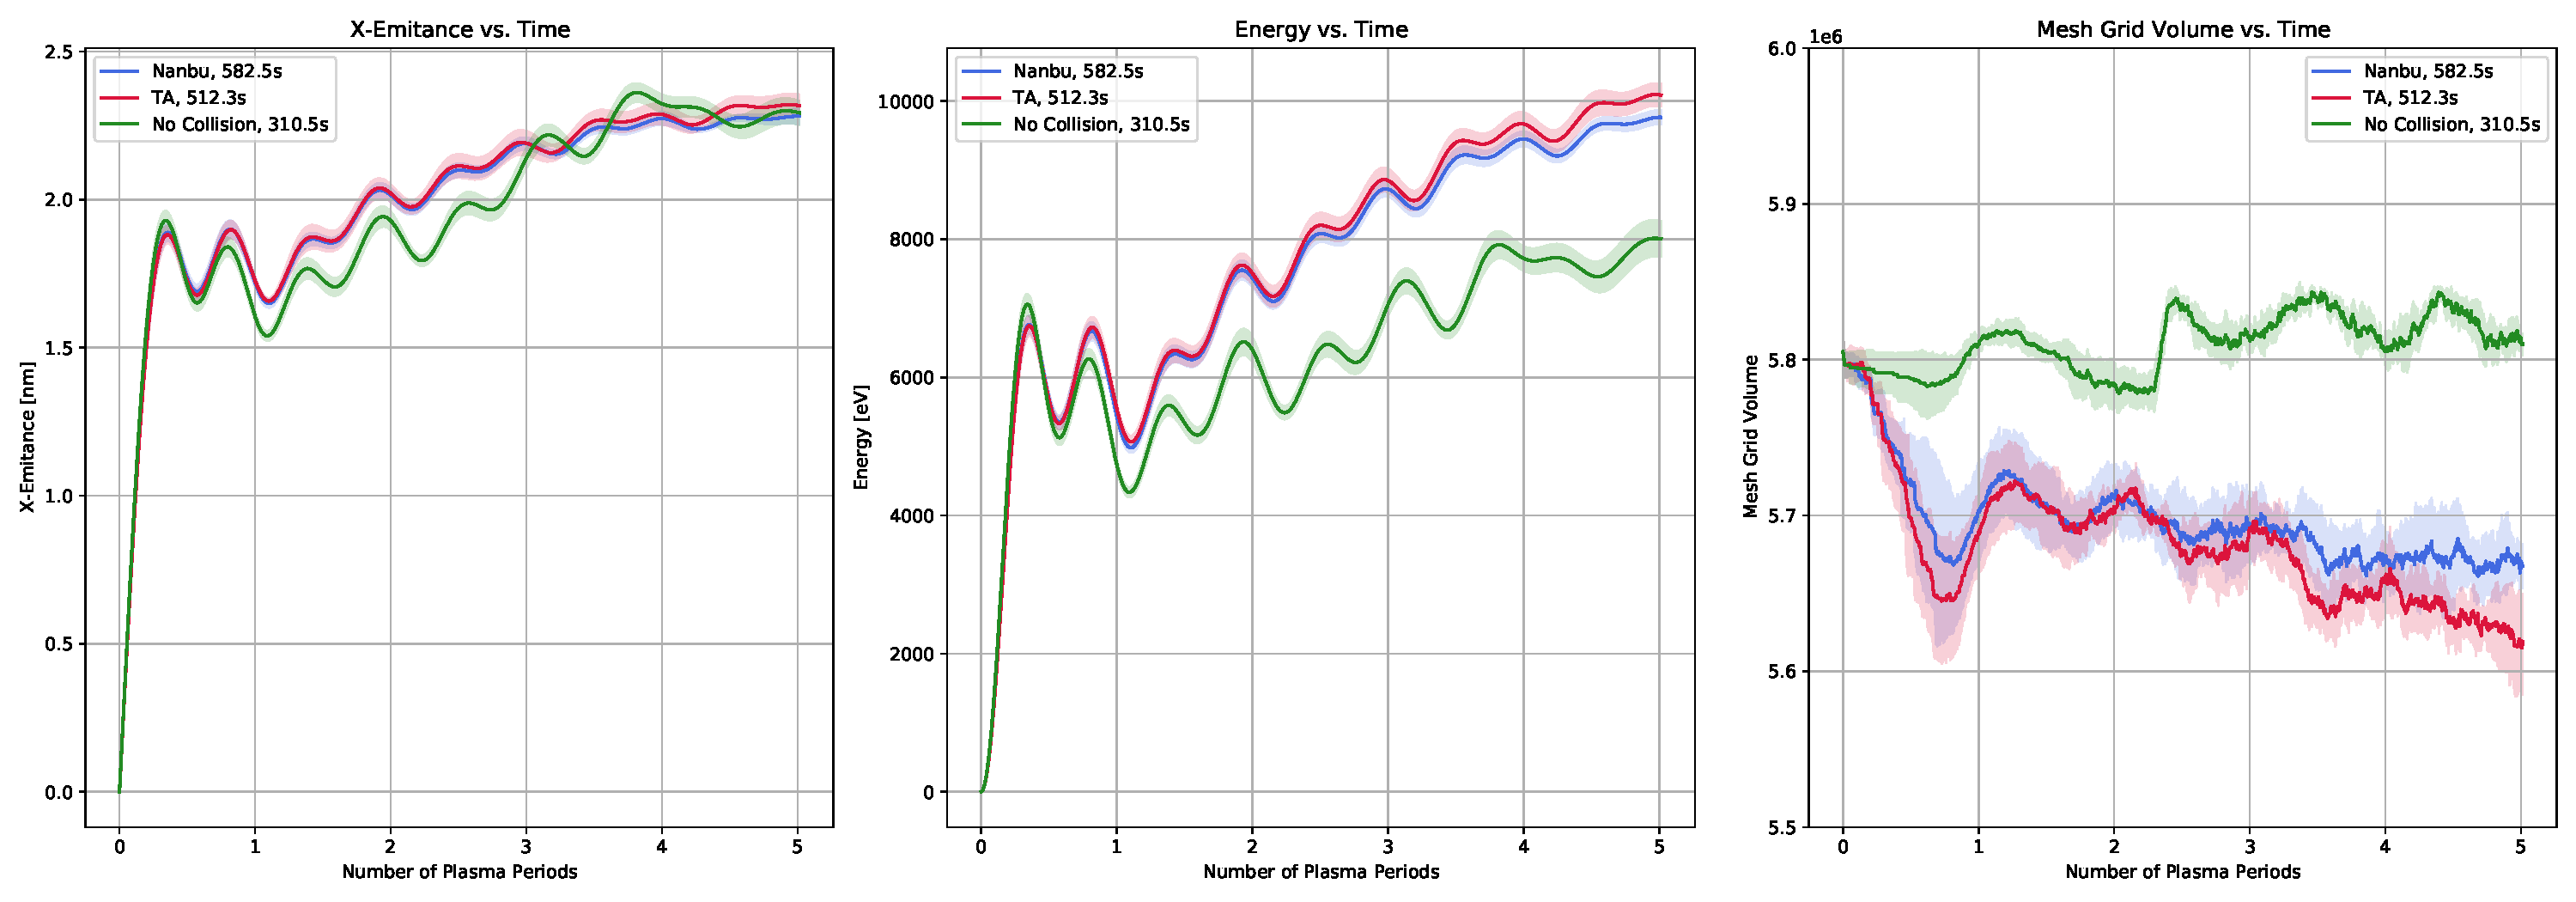
\includegraphics[width=\linewidth]{ressources/test3/cold_sphere_collision_algo_comparison.pdf}
    \captionof{figure}{$x$-emittance, total energy and mesh grid volume against time for different collision algorithms. All simulations were done using $5$ realization with \textsc{Takizuka} and \textsc{Abe}'s collision algorithm. The shaded region denotes the respective standard deviation for the realizations.}\label{img:test3:cold_sphere_collision_algo_comparison}
    \vspace{5pt}
\end{minipage}
%- Has the same effect as \cite[595]{Mitchell2015}: no collisions results in lower emittance
%- However, only slight difference between collision algorithms.
%    --> as mentioned in previous paragraph: only a short period in the beginning of the algorithm were collisions are significant --> small difference in the end, but nice to see that they do make a difference compared to no collisions!
%    --> \textsc{Nanbu} needed $14\%$ longer than TA, but their uncertainties in the emittance overlap: so no statistically significant accuracy increase
%    --> might be different for a test case were collisions are significant all the time (like the \textsc{Trubnikob} test before)
%- \textsc{Nanbu} in this implementation is never faster than TA: simply more calculations without any noticeable accuracy increase
%- However: the algorithm also implements ``\texttt{Nanbu2}'' (does less collisions than the normal \textsc{Nanbu}, but without suffering from worse accuracy) and ``\texttt{Bird}'' (does the minimum necessary number of collisions). For a well conditioned problem, these two might be quite a bit better than TA. But that is not part of this project and only a remnant from the CSP (FS24) lecture project.
The results align with the findings \cite[595]{Mitchell2015}, indicating that the absence of collisions leads to overall lower emittance. However, the differences observed between the various collision algorithms are minimal. As previously mentioned, significant collisions only occur during a brief initial phase of the algorithm, resulting in only slight variations in outcomes. While it is encouraging to see that collisions do influence results compared to scenarios without them, the practical implications are limited. Specifically, the \textsc{Nanbu} algorithm required $14\%$ more computation time than the \textsc{Takizuka \& Abe} (TA) method, yet the uncertainties in the emittance measurements overlap, indicating no statistically significant improvement in accuracy. It is worth noting that the differences in performance might be more pronounced in scenarios where collisions are consistently significant, such as in the \textsc{Trubnikov} test case discussed in \ref{sec:result:trubnikov}. 

In this implementation, \textsc{Nanbu} was never faster than TA, as it involved more calculations without yielding a noticeable increase in accuracy. However, my algorithm implementation also incorporates variations such as ``\texttt{Nanbu2}''—which performs fewer collisions than the standard \textsc{Nanbu} without compromising accuracy (see \cite[7]{Dimarco2010})—and ``\texttt{Bird}'s'' algorithm (see \cite[8]{Dimarco2010}), which executes the minimum necessary number of collisions. For well-conditioned problems, these two alternatives may outperform the TA method significantly. Nonetheless, exploring these variations is beyond the scope of this project and remains a remnant from the CSP (FS24) lecture project.


\subsection{Algorithm Speedup for the Simple Relaxation Test Cases}

% Conduct testcase for both algorithms for some relaxation problem and show simple single-threaded algorithm speedup.
% Additionally, algorithmic speedup in multi-threading when using solver+collisions
The computation times for the single threaded collision executions in figure \ref{img:test1:temperature_diff_dT_combined_shaded} and \ref{img:test1:temperature_diff_N_combined_shaded} can be plotted against the time step size and the number of particles, respectively, in figure \ref{img:test1:computation_time_analysis_single_combined}. \\
\begin{minipage}[h]{\linewidth}
    \vspace{5pt}
    \centering
    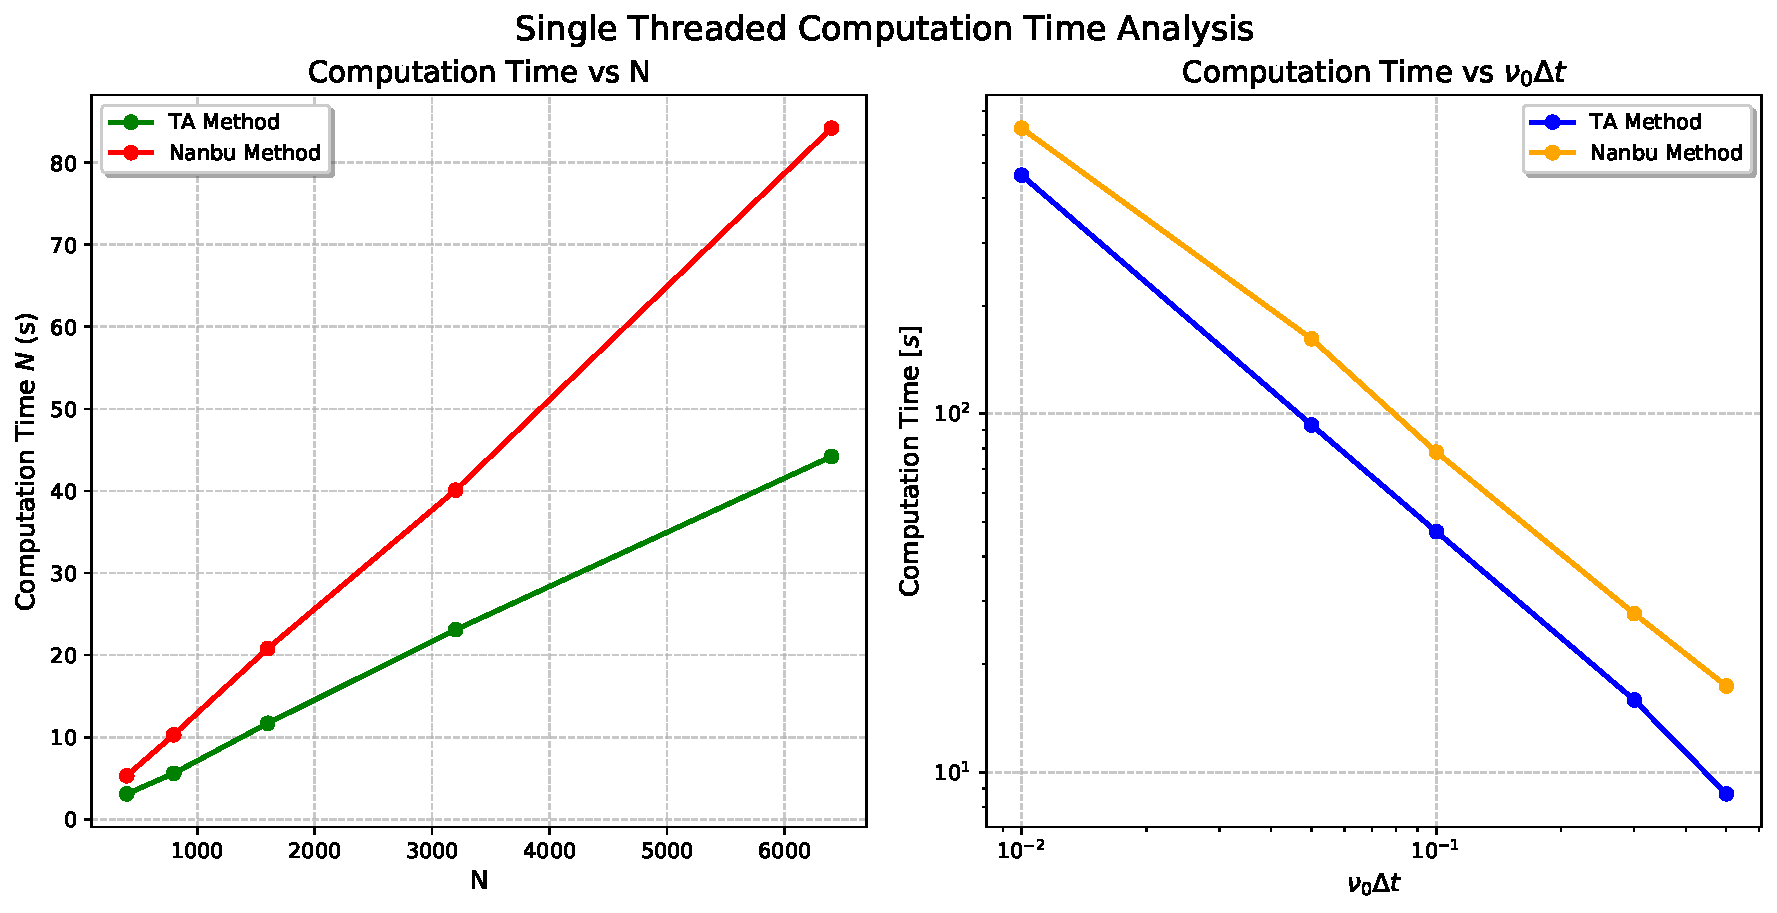
\includegraphics[width=\linewidth]{ressources/test1/computation_time_analysis_single_combined.pdf}
    \captionof{figure}{Computation time plots for varying number of particles and varying time step sizes. The right plot has logarithmic axis, the left one is linear. }\label{img:test1:computation_time_analysis_single_combined}
    \vspace{5pt}
\end{minipage}
One can see that the collision computation time increases linear with the number of particles, which makes sense, since double the particles means double the number of collision function calls. For the logarithmic time step size plot, a linear fit to the values reveals a slope of almost exactly $-1$. This is also expected, since the number of time steps increases anti proportional to the time step size, while the computation time increases linearly with the number of time steps. 

% TODO: maybe multi threaded???
\textbf{Multithreaded Computation.} The whole program can successfully compile using OpenMP as well as CUDA. However, running the program is potentially limited:
\begin{description}
    \item[OpenMP] \hfill \\
    It does compile and I ran it successfully on 4 and on 2 threads\footnote{This is due to the limitation of my laptop. Euler was at the time not available, since some required dependencies were removed after a operating system change.} and even saw some speedup. Since $4$ cores utilizes my CPU $100\%$, it got slowed down at that point. But from 0 to 2 cores, I got an average of $29\%$ speedup. \\
    However, the multithreading currently does not work together with the adaptive mesh sizing. The problem seems to be what I mentioned before: since the program uses many different methods to ``normalize using domain size'', it is not easy to change every appearance of things like \texttt{.setGridSize()} or \texttt{rmax\_m}. Currently, the program always crashes during \texttt{.accumulateHalo()} (it only ran once or twice by chance through that function -- likely because there were no particles in the halo).

    \item[CUDA] \hfill \\
    I managed to compile the code and successfully run it for a few iterations. However, there is inevitably an error stating: 
    \begin{verbatim}
cudaDeviceSynchronize() error( cudaErrorIllegalAddress): an illegal 
memory access was encountered /home/.../ippl\_build/kokkos/
kokkos-4.1.00/core/src/Cuda/Kokkos\_Cuda\_Instance.cpp:139
    \end{verbatim}
    It seems to already happen during the initial \texttt{.pre\_run()} before even calling the \texttt{initializeParticles()}. Sadly, I was not able to fully run the program yet.
\end{description}


\section{Conclusion}

%- Bigger dataset for error analysis in Trubnikov test
%- 
The project successfully implements the DSMC method for simulating plasma relaxation, providing  insights into the performance of different collision algorithms. The \textsc{Takizuka} \& \textsc{Abe} method was found to be more computationally efficient than \textsc{Nanbu}'s algorithm without significant loss of accuracy, even though \textsc{Nanbu} is the newer version. However, alternative variations like ``Nanbu2'' and ``Bird'' algorithms suggest potential improvements (those are not studied here, but can be used with the provided code \cite{aliemen2024}), which were beyond this project's scope. The scalability of the implementation is promising, although challenges remain in optimizing CUDA-based computations due to current limitations. \\
To further the study, it would be beneficial to expanding the dataset for more comprehensive error analysis. Especially the \textsc{Trubnikov} test would benefit from more data points. Another important improvement would be the revision of the domain customization to avoid inconsistencies and possibly take full advantage of multi threading.

Overall, this means that there is still room for improvement in the code. For the most part, however, the test cases were successfully executed and solved, which allowed the algorithms to be examined sufficiently.



 % Outsourcing text makes the whole thing clearer

\newpage % TODO remove later...
\vspace{2cm}
\printbibliography % Bessere Quellenangabe!

% ----------------------------------------------------------------
\newpage
\thispagestyle{empty}
\newpage 
\appendix % Appendix begins here...

\section{Appendix}

\subsection{General Compile Instructions}

I used the following software:
\begin{itemize}
    \item IPPL version: \texttt{V3.0.1}.
    \item Modules: \texttt{gcc/11.4.0}, \texttt{cmake/3.26.3}, \texttt{cuda/12.2.1}, \texttt{openmpi/4.1.4}.
    \item Tested GPU Architecture: GPX1050, PASCAL61.
    \item Used CPU: Intel Core i7-7700HQ (4 cores, 8 threads).
    \item Operating system: Windows 10, IPPL was used in the Linux Subsystem for Windows.
\end{itemize}
I used the \texttt{999-build-everything} script provided by IPPL to compile everything. For example:
\begin{verbatim}
    ippl-build-scripts/999-build-everything -t serial -k -f -i -u 
    ippl-build-scripts/999-build-everything -t openmp -k -f -i -u 
    ippl-build-scripts/999-build-everything -g PASCAL61 -t cuda -k -f -i -u 
\end{verbatim}
More instructions can be found in the GitHub repository with the code under \cite{aliemen2024}.

%TODO
%- Code is here...: 
%- Put code into folder: ....
%- Run like this and that for different testcases: ...
%- Used IPPL version 3.2.0, newer had problem with \texttt{hefte\_fft3d.h} and older didn't find Kokkos or somethin like that...
%- Coulomb logarithm: \url{https://farside.ph.utexas.edu/teaching/plasma/Plasma/node39.html}
%- Problem: only works for rho 1/NParticles in the beginning, even though later stages calculate NParticles/1...?!?!?!?!
%TODO


\subsection{Potential Problems and Bugs}

A list of potential problems and bugs:
\begin{itemize}
    \item There is a problem with applying the boundary conditions for very fast particles. When the boundaries are from $0$ to $L$ and the particle position is for example $>2*L$, then the particle will still not land inside the domain. Instead of calculating the modulo, only ``one domain size'' is subtracted. I fixed it by implementing my own boundary check in \texttt{applyExtendedBC()}.
\end{itemize}


\subsection{Old Cold Sphere Results}

For the presentation in the CSP lecture (FS24), we presented figure \ref{img:additional:disorder_heating_grid_comparison}. \\
\begin{minipage}[h]{\linewidth}
    \vspace{5pt}
    \centering
    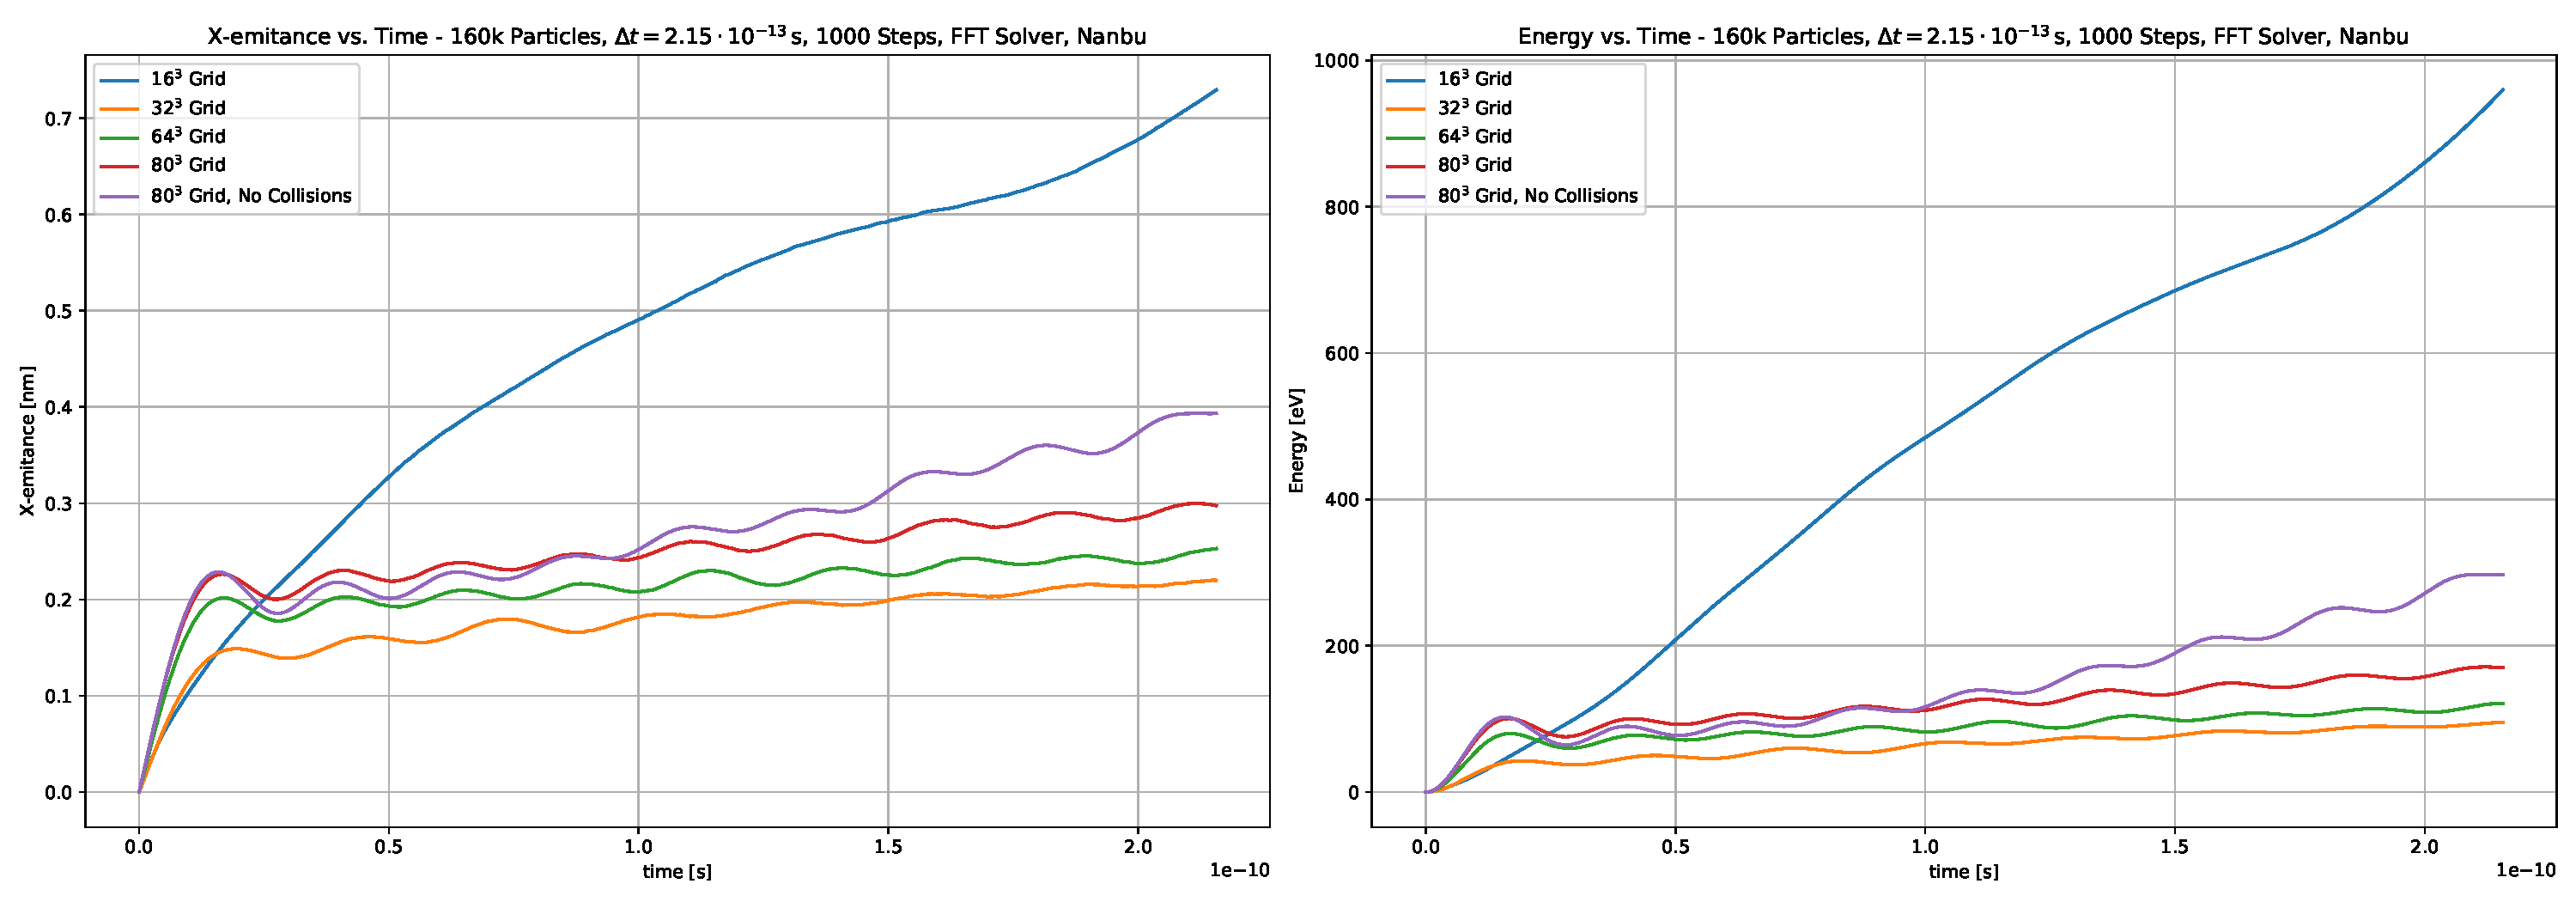
\includegraphics[width=\linewidth]{ressources/additional/disorder_heating_grid_comparison.pdf}
    \captionof{figure}{$x$-emittance and total energy against time for different mesh grid sizes.}\label{img:additional:disorder_heating_grid_comparison}
    \vspace{5pt}
\end{minipage}
The simulation was done using $156055$ particles and \textsc{Nanbu}'s collision algorithm.
 % appendix contents file
% ----------------------------------------------------------------
% Anhang (Messprotokoll)
%\newpage
%\pagestyle{trueempty} % Deaktiviere Header
%\addcontentsline{toc}{section}{Appendix}
%\pagestyle{trueempty}
%\includepdf[scale=0.9, pages={1}, pagecommand=]{ressources/protocol.pdf} % empty "pagecommand" to enable "Appendix" title...


\end{document}